%%%%%%%%%%%%%%%%%%%%%%%%%%%%%%%%%%%%%%%%%%%%%%%%%%%%%%%%%%%%%%%%%%%%%%%%%%%%%%%%%%%%%
% Machine Learning in Control
%
% 1. Reinforcement learning Q-learning algorithm
%  - Extension to of tabular methods to continuous processes using interpolation
%  - Can be extended further using neighbourhood information
% 2. Continuous control using deep reinforcement learning
% 3. Comparison of results with MPC on simple systems
% 4. Fault tolerant RL vs. traditional methods
% 5. Control of a wastewater treatment process
% 6. Optimization
%  - Adaptive using model updates
% 
%%%%%%%%%%%%%%%%%%%%%%%%%%%%%%%%%%%%%%%%%%%%%%%%%%%%%%%%%%%%%%%%%%%%%%%%%%%%%%%%%%%
Advanced process control and optimal control have traditionally used mathematically programming based trajectory optimization methods \cite{empc2, zone_mpc, mpc, empc1,}.  The effectiveness of these methods in addressing multi-stage optimal control problems have been widely demonstrated; however, industrial scale application of such methods in stochastic multiple-input multiple-output (MIMO) systems are still limited due to design and computation complications \cite{MS}. For example, accurate model identification of complex MIMO non-linear systems are nearly impossible. Even if a model were to exist, the computational cost for the non-linear program could be infeasible for online applications. Furthermore, the optimized trajectory to systems containing uncertainty use stochastic programming with only a finite number of uncertainty scenarios and uncertainty information is assumed to be known. In practice, such information are typically unknown, non-stationary and are uncertain themselves \cite{jayCCE}. Moreover, the prediction and control horizon of the trajectory optimization for large MIMO systems are generally truncated to ensure feasible computation time. Though, the identified optimal trajectory for short horizons are typically local optimal solutions \cite{mpc}. Lastly, MP methods require accurate dynamical system models (although no models are perfect in real life); intuitively bottlenecking the optimality of the solution, a scenario similar to supervised learning.

Comparatively, RL online computational times are significantly shorter even for long control horizons or large-scale MIMO systems because the optimal solutions are pre-computed and stored offline, a concept similar to explicit model predictive control (MPC) where parametric programming is used \cite{explicit_MPC}. Furthermore, RL finds the optimal policy through meaningful interactions with the environment.  After each interaction, values are assigned/updated for the visited state. The value functions are stored for future decision making.  Through this identification process, the value functions implicitly contain the uncertainty information of all $x \in \mathcal{X}$. From these unique features of RL in control applications, it is a natural curiosity to explore its potential in the process control industry.

The contributions made in this chapter are as follows:
\begin{enumerate}
    \item Introduction of a simple, cost-effective, and explainable RL algorithm for process control.  The method is also continuous and non-linear.
    \item Compared RL and deep RL to traditional optimal control methods such as MPC.
    \item Applied RL to an industrial grade waste water treatment plant (WWTP) for optimal control.  Results were compared to MPC, economic MPC, and distributed MPC frameworks.
    \item Applied RL for fault prediction and fault tolerant control applications.
\end{enumerate}


\section{An direct adaptive optimal control method}
On a high level, optimal control methods extremize the functional equation of a system through MP methods. In literature, it was found that optimal control methods are less tractable both computationally and analytically compared to set-point tracking or regulations methods (due to non-convex optimization among factors). Consequently, adaptive optimal control methods have received less academic attention, with most existing studies focused on indirect methods like model re-parameterization \cite{rl_control}.  In \cite{rl_control}, RL was shown to be an effective \textit{direct} optimal control method as it adapts its control policy directly. Direct adaptive optimal control methods are especially useful for systems where accurate models are not identifiable and/or available.  In such scenarios, in-direct methods struggle because the accuracy of the model is paramount for successful control.  On the other hand, direct methods can update the control policy directly through interactions with the system, eventually arriving at the optimal policy. In \cite{power_control}, the authors showcased RL's directly adaptive nature by applying an agent onto the control system of a data-center cooling application. In such systems, accurate models are nearly impossible to identify due to complex non-linear relationships between thousands of variables. However, the agent here was able to adapt to the optimal policy directly after sufficient online interactions which ultimately resulted in 22\% reduced power consumption compared to model-based approaches.  Likewise, \cite{power_control2} applied RL onto power systems with ever-changing load fluctuations.  Again, such a system is nearly impossible to model through traditional means; however, the agent was still able to adapt its policy after sufficient online interactions. Wireless networks is a third system with nearly unidentifiable dynamics. The authors in \cite{power_control3} demonstrated deep RL's direct adaptive nature through its application onto wireless networks, ultimately resulting in superior control compared to all previous methods.

\section{Controlling a VFD using $Q$-learning}
A detailed quantitative example is provided in this section to serve as a gentle introduction of RL's applicability in process control systems \footnote{For further intuition, the supplementary code for all results generated in this section are located at: https://github.com/RuiNian7319/Research/tree/master/2.RL\_Codes/Mechatronix}. Here, the \textit{off-policy} tabular $Q$-learning algorithm with upper confidence bound (learning acceleration heuristics) was used for output pressure tracking of an industrial variable frequency drive (VFD) pump. 

\subsection{System Description}
The industrial VFD system is built by Turbine Technologies and is called the FLUIDMechatronix.  On the system, there exists thousands of different tags measuring countless states. For this control example, the output pressure, $P_{out}$, and pump RPM will be used. From the FLUIDMechatronix manual, the safe operating ranges of the pressure and pump RPM are:
$$0 \; kPa \leq P  \leq 45 \; kPa$$
$$0 \; Hz \leq RPM  \leq 60 \; Hz$$
In terms of system representation, a FOMDP will be used because all system measurements are available and the system dynamics are fast. Initially, the system starts in:
\begin{equation}
    P_0 = 41 \; kPa
    \label{eq:initial_p}
\end{equation}
\begin{equation}
    u_0 = 60 \; RPM
    \label{eq:initial_u}
\end{equation}

\begin{figure}[H]
    \centering
    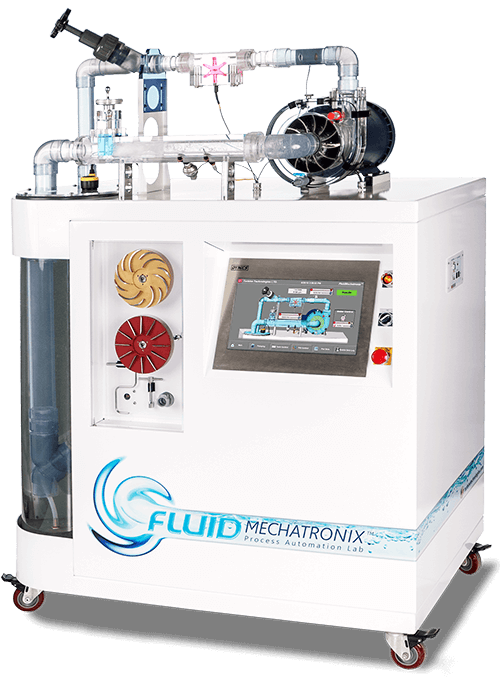
\includegraphics[width=0.38\textwidth]{images/ch4/Mechatronix.jpeg}
    \caption{The FLUIDMechatronix experiment from Turbine Technologies \cite{turbine}.}
    \label{fig:mechatronix}
\end{figure}

Implementing RL for the control of an industrial process typically involves four steps: i) Model identification; ii) agent design; iii) initial training; iv) online calibration.  The details of each step are shown in \ref{fig:rl_implementation}.

\begin{figure}[H]
    \centering
    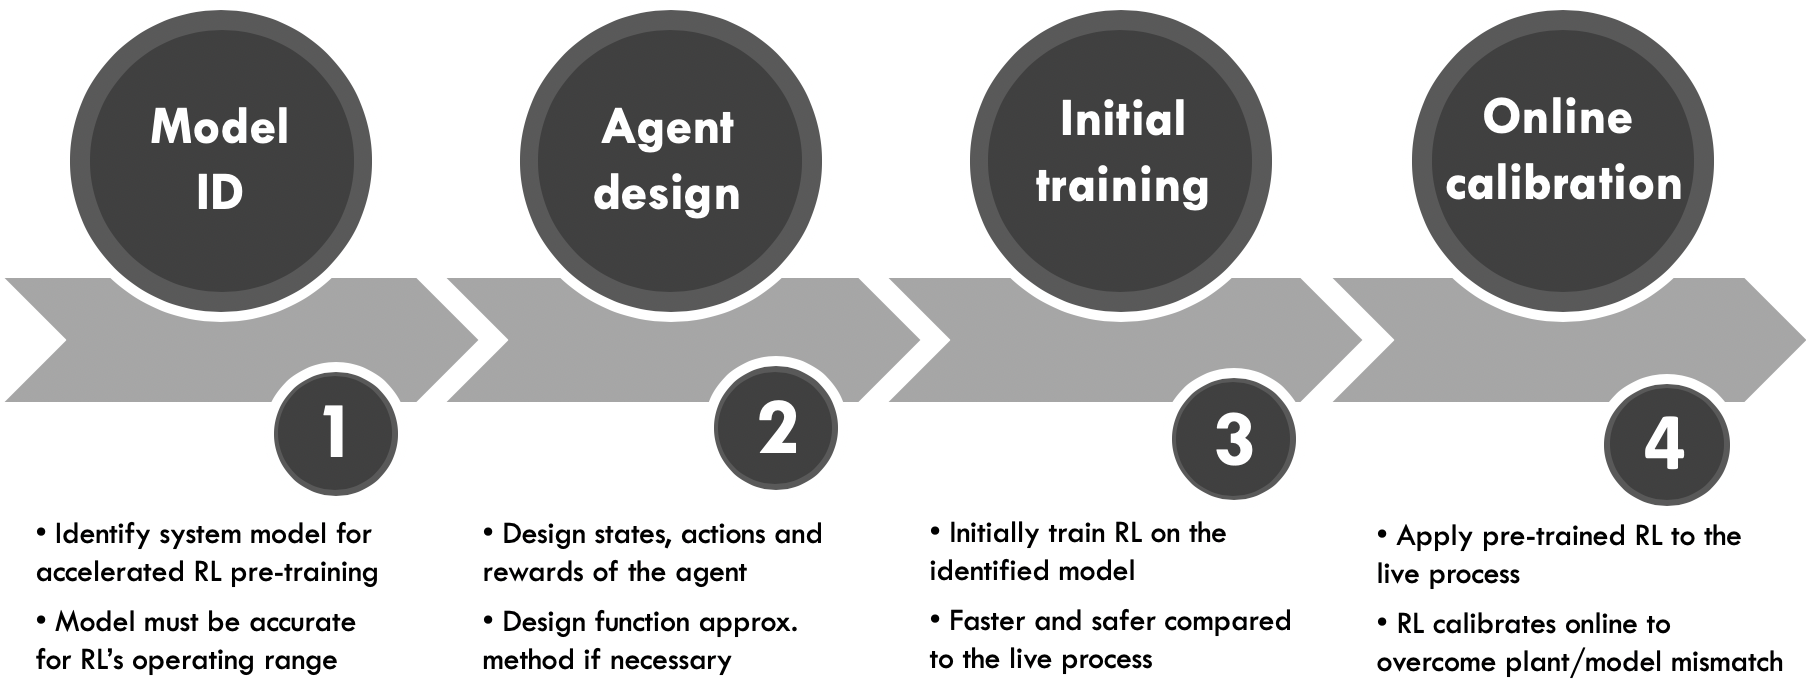
\includegraphics[width=0.95\textwidth]{images/ch4/RL_implementation.jpeg}
    \caption{General procedure for implementing industrial reinforcement learning.}
    \label{fig:rl_implementation}
\end{figure}

\subsection{Step 1: Model ID}
One major drawback of RL is its unreasonable data efficiency.  In fact, it \textit{may} take thousands of interactions before anything meaningful is first learned.  As such, implementing RL to learn online is time-infeasible because decades may pass before the optimal policy is identified.  To overcome this flaw, a \textit{representative} simulation model can first be constructed to pre-train the agent offline.  After adequate performance is observed in simulation, the agent can be implemented online.  Initially, the agent will calibrate its policy to the live process to overcome any model-plant mismatches. The time required for calibration is heavily dependent on the accuracy of the simulation model.  For perfectly representative models, such as video games, a calibration time is not required. Afterwards, optimal control can commence.

For model identification, pseudo-random input signals were used to provide excitation to the VFD for input-out data generation. The data collection process was terminated after 18,000 input-output signals were obtained. Then, a quadratic model was identified using least squares. The identified model is given as:
\begin{equation}
    P_{out} = 0.012 \cdot RPM^2 + 0.024 \cdot RPM - 2.073
\end{equation}
The mean squared error (MSE) of the identified model was 0.056 and the fitted model compared to the experimental data is shown in Figure \ref{fig:04model_fit}.
\begin{figure}[H]
    \centering
    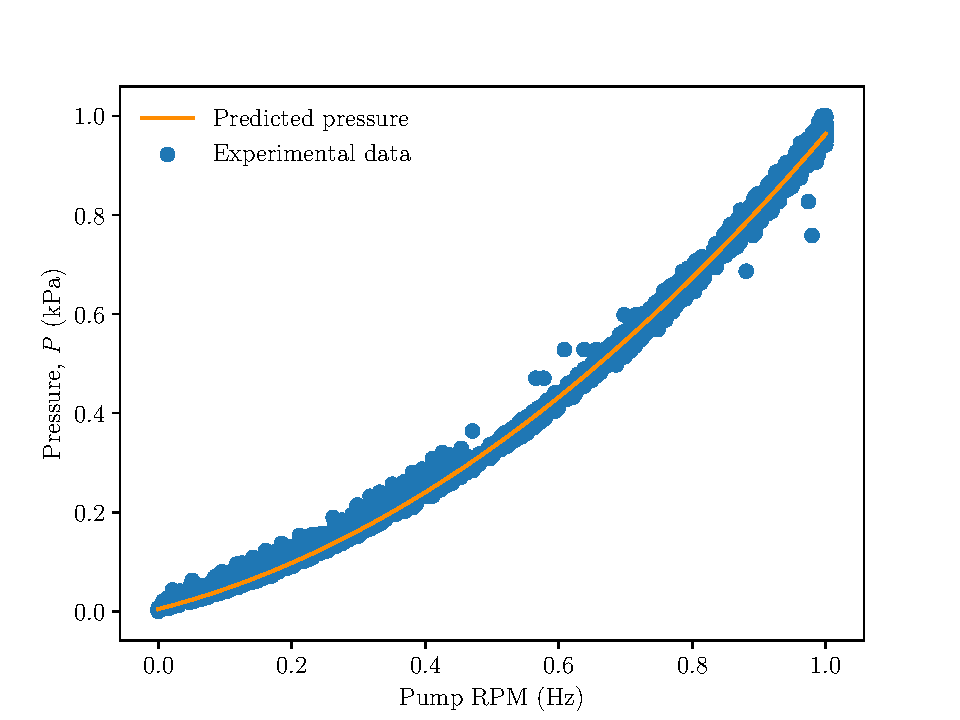
\includegraphics[width=0.7\textwidth]{images/ch4/model_fit.pdf}
    \caption{Performance of the identified system model on a test data set.}
    \label{fig:04model_fit}
\end{figure}

\subsection{Step 2: Agent design}
The overall RL paradigm for this example is shown in Figure \ref{fig:04rl_system1}. Intuitively, the agent tracks a set-point for the output pressure by manipulating the pump RPM.  To allow for the tracking of a variable set-point, the state of the agent is the current tracking error:
\begin{equation}
    \varepsilon = P_t - P_{t, sp}
\end{equation}
and the action is the \textit{change} in pump RPM $\Delta u$. Here, $P_t$ is the pressure at time $t$ and $sp$ denotes the set-point. This \textit{velocity} based implementation is a requirement for tracking multiple set-points. If the action was the pump RPM instead (and not $\Delta u$), then the agent would fail to track multiple set-points since it simply maps different tracking errors to one pump RPM that corresponds to \textit{one} set-point. For example, suppose the current set-point is $10 \; kPa$ and $P_t = 0$ resulting in a -10 tracking error. Here, suppose the optimal RPM is $u = 20$. After implementing $u = 20$, the system reaches steady state and achieves a tracking error of 0. After some time, the machine operator may then decide to change the set-point to $20 \; kPa$. Now again, the tracking error is -10; however, the RPM from the agent would still be $u = 20$ because the state-action is a 1 to 1 mapping; thus, unable to track any changes in set-points. 

The reward function of the agent is given by:
\begin{equation}
    r(x, u) = max(-\varepsilon^2 - \Delta u, -200)
\end{equation}
where $\Delta u$ is the change in input to discourage the agent from making unnecessary actions. Additionally, the reward is clipped to -200 for convergence properties and to avoid numerical issues as explained in the reward clipping section. The upper reward limit is not clipped because the function is naturally capped at 0. Here, the agent evaluates every five seconds to guarantee that steady state has been reached before consecutive actions are made. Five seconds was chosen because it was identified to be the longest transition time required. Moreover, the decision making would not be Markovian (i.e., observed states are not independent of the past because the states do not provide the transition information to the agent) if the agent evaluates during the transition period. In such scenarios, the agent will fail to learn anything meaningful. 

\begin{figure}[H]
    \centering
    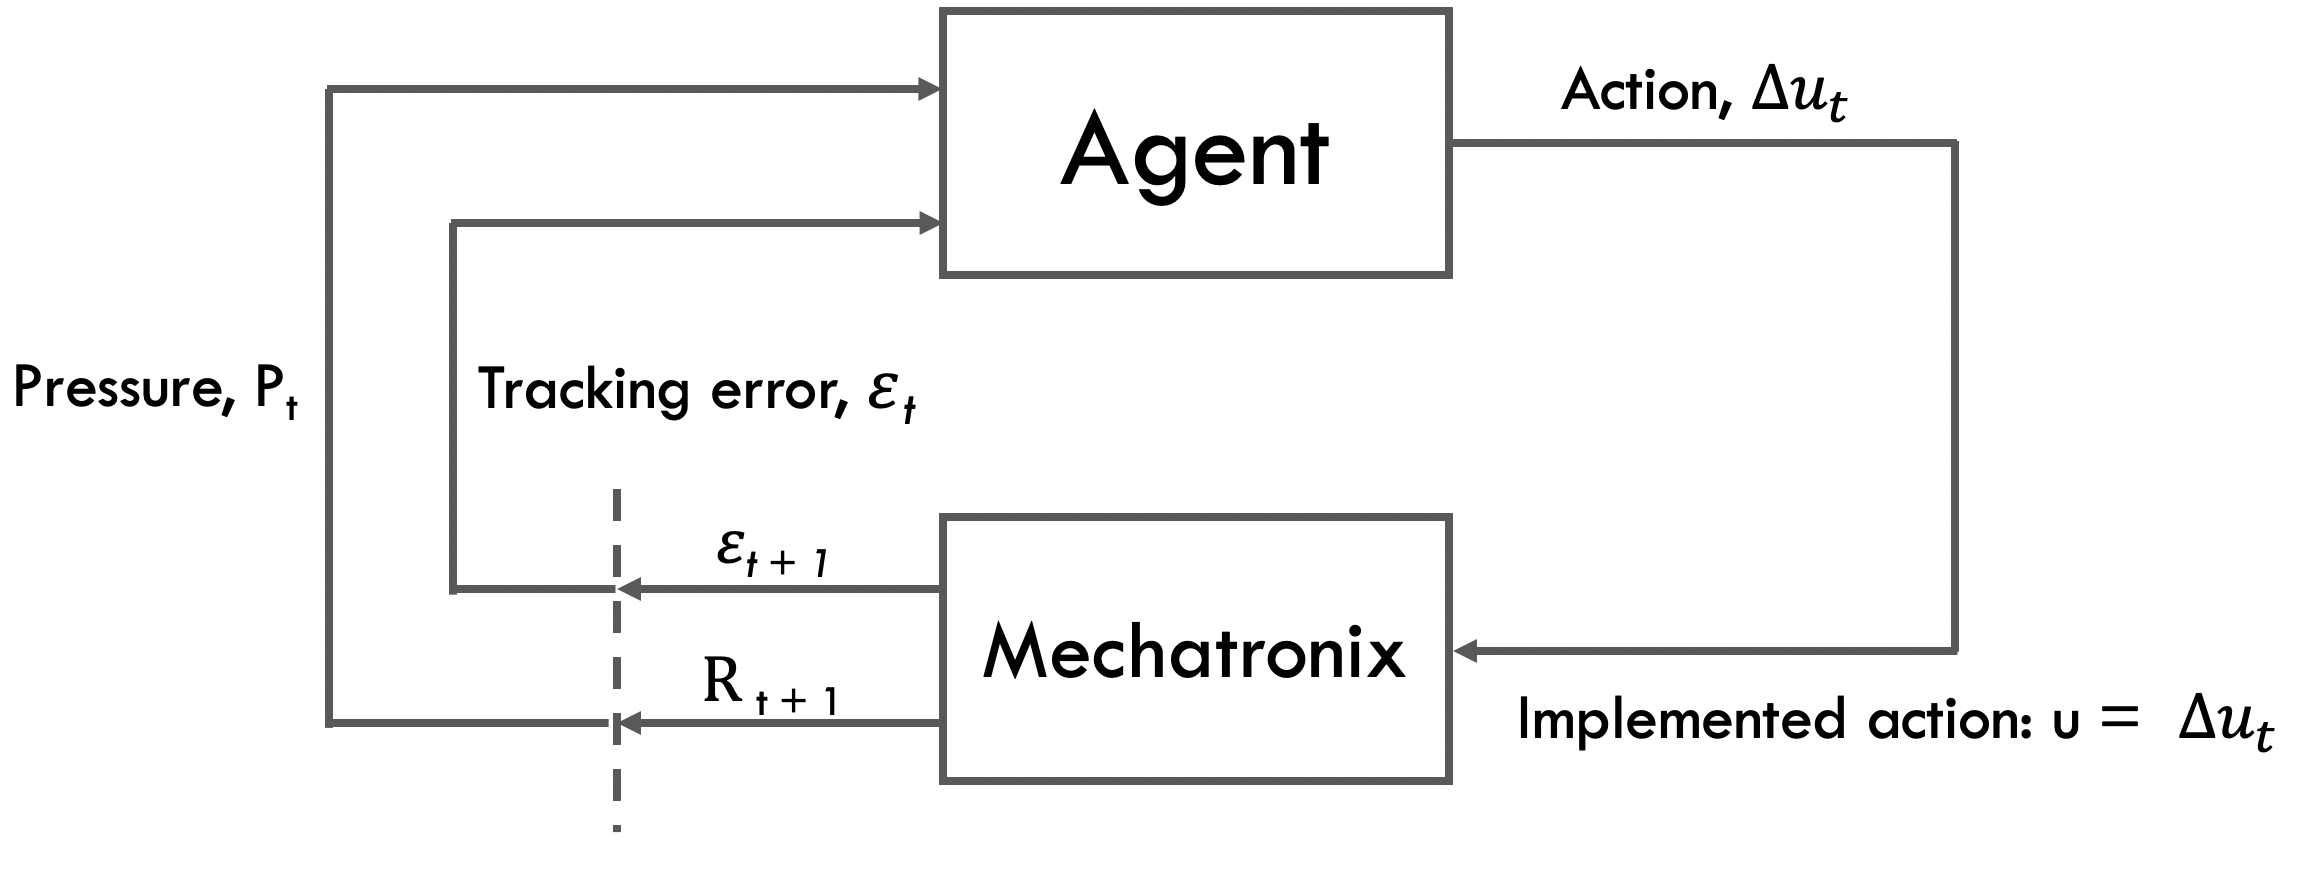
\includegraphics[width=0.7\textwidth]{images/ch4/rl_system1}
    \caption{The RL set-up for the FLUIDMechatronix experiment.}
    \label{fig:04rl_system1}
\end{figure}

All hyper parameters of the agent are shown in Table \ref{tab:rl_system1_params}. The states and actions of the agent are discretized as:
\begin{equation}
    x = [-20, -19, ..., 20]_{1 \times 41}
\end{equation}
\begin{equation}
    u = [-10, -9, ..., 10]_{1 \times 21}
\end{equation}
totalling 861 different action-values to identify. Furthermore, the $Q$-matrix storing all the action-value functions is shown in Figure \ref{fig:q_matrix_system1}.  The agent is initiated with all action-values as 0, a condition known as \textit{tabula rasa}.
\begin{figure}[H]
    \centering
    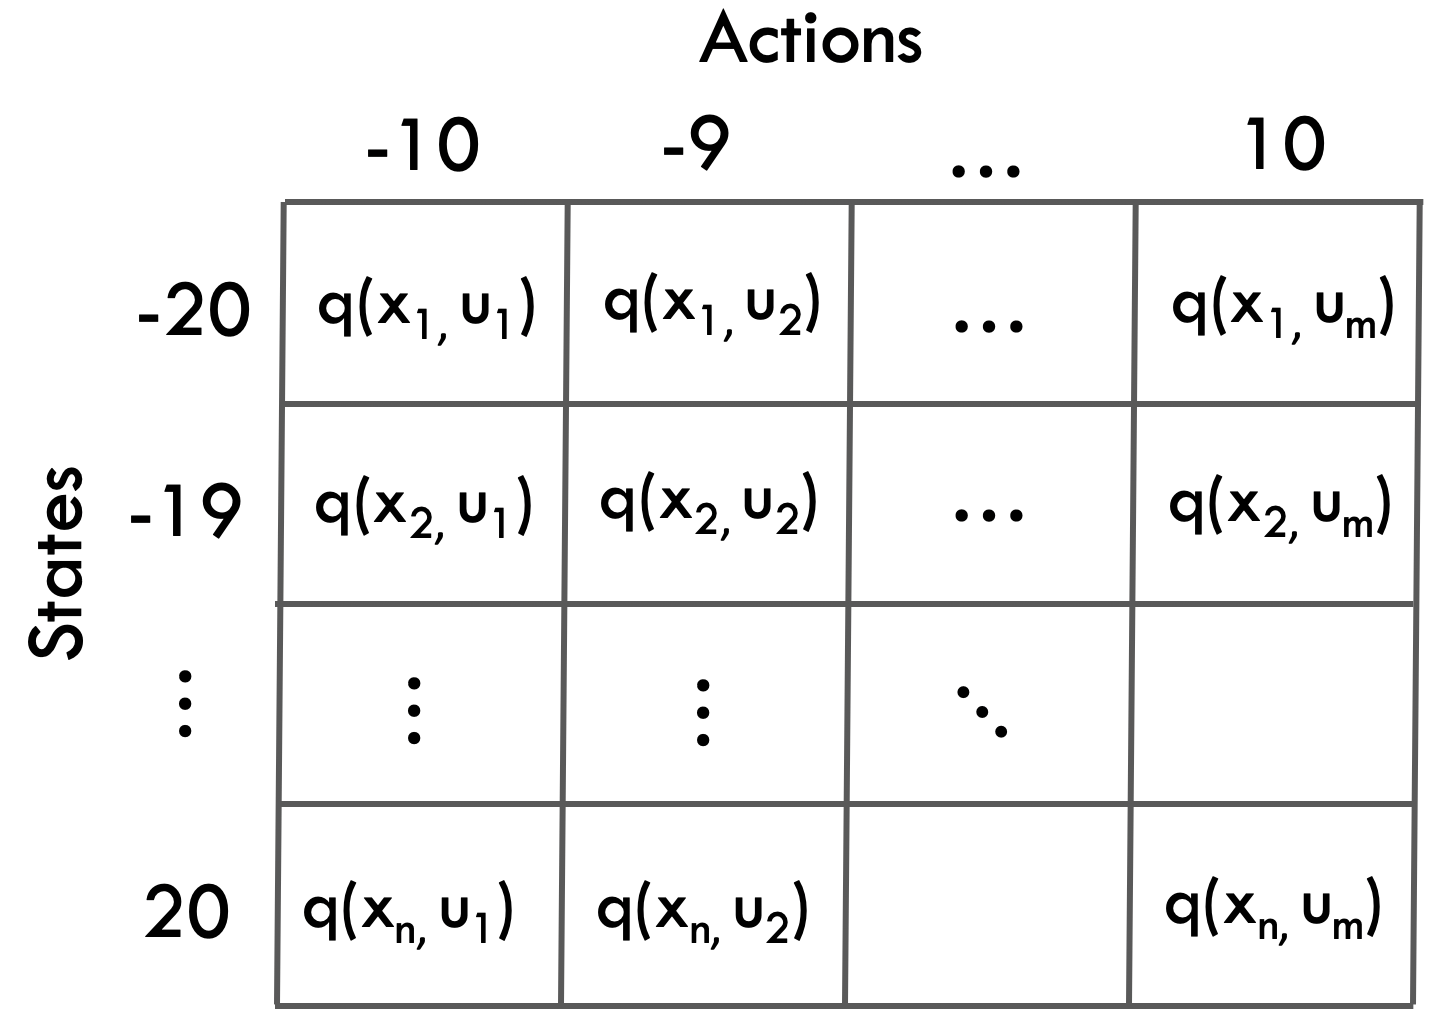
\includegraphics[width=0.5\textwidth]{images/ch4/q_matrix_system1.jpeg}
    \caption{$Q$-matrix of the Mechatronix system.}
    \label{fig:q_matrix_system1}
\end{figure}
The states and actions on the axis of the $Q$-matrix correspond to $\varepsilon$ and $\Delta u$, respectively.  The discount factor, $\gamma$, was 0.9. Altogether, 2,000,000 time steps were used to train the agent (corresponding to 115.7 days of continuous operating experience). After every 400$^{th}$ time step, the agent's state and action was reset back to Equations \ref{eq:initial_p} and \ref{eq:initial_u} to prevent extreme controller saturation. 

The agent uses a equiprobable random exploratory policy ($\epsilon$ = 1) to conduct initial exploration. Throughout training, $\epsilon$ is slowly and linearly decayed until $\epsilon = 0.1$ by the 500,000$^{th}$ update. Likewise, the learning rate is initiated at 0.7 and also linearly decay until 0.001.

\begin{table}[H]
\caption{Summary of the agent's hyper parameters in the Mechatronix experiment.}
\label{tab:rl_system1_params}
\centering
\begin{tabular}{c|c}
\textbf{Hyper Parameter}     & Value  \\
\hline
States, $x$	             	& $\varepsilon = [-20, -19, ..., 20]_{1 \times 41} $		 \\
Actions, $u$               & $\Delta u = [-10, -9, ..., 10]_{1 \times 21}$		\\
Reward, $r$	               & max($-(\varepsilon^2 + \Delta u)$, -200)		\\
Learning rate, $\alpha$		& [0.001, 0.7]		 \\
Discount factor, $\gamma$      	& 0.9  \\
Exploratory factor, $\epsilon$             & [0.1, 1]  \\
Evaluation time                 & 5 seconds \\
System representation           & FOMDP \\
\end{tabular}
\end{table}

\subsection{Step 3: Initial training}
The agent behave as follows: the agent observes some initial tracking error $\varepsilon_t$ and performs a random action $\Delta u_t$ with accordance to its behaviour policy (initially equiprobable random).  Next, the pump RPM corresponding to $u_t = u_{t-1} + \Delta u_t$ is sent to Mechatronix.  After five seconds, the agent receives reward $R_{t+1}$ and then observes new tracking error, $\varepsilon_{t+1}$. Using the tuple $(x_t, u_t, r_{t+1}, x_{t+1})$, the agent updates its current knowledge via Equation \ref{eq:q_learning}. This step is repeated many times until the optimal policy, $\pi^*$, is identified. A numerical walk-through of the calculations is shown below:

\begin{quote}
    Suppose another simpler agent was constructed for this system. For this agent, the system was discretized into five states and three actions:
    $$x = [-21, -10, 0, 10, 21]_{1 \times 5}$$
    $$u = [-1, 0, 1]_{1 \times 3} $$
    Consequently, the $Q$-matrix was initialized as:
    
    $$ Q(x, u) = \left(\begin{matrix}   0 & 0 & 0 \\
                                        0 & 0 & 0 \\
                                        0 & 0 & 0 \\
                                        0 & 0 & 0 \\
                                        0 & 0 & 0 \end{matrix}\right) $$
    
    where the rows and columns correspond to the different states and actions, respectively. The system's set-point was initially at 30 kPa. The agent was initiated at steady state with 15 kPa and 37 RPM, resulting in $\varepsilon=-15$. At $t = 0$, the agent receives the error and rounds it to the nearest discretized value, $x = -10$.  Given this state, the agent uses the $Q$-table and picks the action that corresponds to the highest $Q$ value (note if a equiprobable random policy was initially followed, a random action would be selected instead):

        $$Q(-10, u) = [0, 0, 0]$$

    where the three values correspond to the predicted action-values for selecting actions $\Delta u = -1, 0, -1$, respectively. Since the agent is inexperienced and have not been provided with prior information about the system, it thinks that all three actions are indifferent; therefore, the agent will pick an arbitrarily action to learn more about the system. Moreover, during scenarios where $Q^{max} = Q_1 = Q_2 = ... = Q_n$, ties \textit{must} be broken arbitrarily to avoid biasing one action over all others.
    
    Assuming that $u = -1$ was picked, the system will transition to 13.8 kPa. After five seconds, the new observed tracking error would be -16.2. Clearly, this was a sub-optimal action; if the pressure was already lower than the set-point, it would be intuitive to increase pump RPM instead. However, a \textit{tabula rasa} agent is not aware of such a phenomenon, humans only know this through prior experience. Here, the agent would also receive reward:
    $$max(-16.2^2 - 1, -200) = -200$$ 
    and be in new state $x_1 = -21$.  From this interaction, the agent would then update the $Q$-matrix using Equation \ref{eq:q_learning}:
    $$Q(-10, -1) \leftarrow Q(-10, -1) + 0.7 [-200 + \gamma Q(-21, 0) - Q(-10, -1)]$$
    $$Q(-10, -1) \leftarrow 0 + 0.7 [-200 + 0.9 \cdot 0 - 0]$$
    $$Q(-10, -1) \leftarrow -140 $$
    and the updated $Q$-matrix would be given as:
    
    $$ Q(x, u) = \left(\begin{matrix}   0  &  0  & 0 \\
                                        -140 & 0 & 0 \\
                                        0 & 0 & 0 \\
                                        0 & 0 & 0 \\
                                        0 & 0 & 0 \end{matrix}\right) $$
                                        
    In this case, all three $u$'s for $Q(x_{t+1}, u_{t+1})$ are also reward maximizing; therefore, the ties are here must also be broken randomly to avoid unnecessary bias. Suppose the system was reset, initiating at $x_0 = -10$.  This time, the $Q$-matrix provides:
    
    $$Q(-10, u) = [-140, 0, 0]$$
    
    telling the agent that $\Delta u = -1$ is a sub-optimal compared to $\Delta u = 0 \text{ or } 1$.  For a reward maximizing agent, either $\Delta u = 0 \text{ or } 1$ would be picked instead.  
    
    After many interactions with the system, the $Q$-matrix now becomes:
    
        $$ Q(x, u) = \left(\begin{matrix}   -152  &  -133  & -120 \\
                                        -149 & -121 & -99 \\
                                        -31 & -22 & -33 \\
                                        -102 & -142 & -162 \\
                                        -152 & -162 & -177 \end{matrix}\right) $$
    
    Now, the agent has vastly more knowledge about the system and can begin acting optimally. After resetting the agent back to $x_0 = -10$, the decision making of the agent is now deterministic.  The corresponding action-values given $x_0 = -10$ are:
    
    $$Q(-10, u) = [-149, -121, -99]$$
    
    Here, the agent would pick $\Delta u = 1$ corresponding to $Q(-10, 3) = -99$ (greedy action) and the system would transition to $P_1 = 16 \; kPa$.  Although the error is still closest to -10 (set-point is 30 kPa), the reward obtained is much better compared to actions -1 or 0.  The new update step is given as:
    
    $$Q(-10, 1) \leftarrow Q(-10, 1) + 0.001 [-197 + \gamma Q(-10, 1) - Q(-10, 1)]$$
    $$Q(-10, 1) \leftarrow -99 + 0.001 [-197 + 0.9 \cdot -99 + 99]$$
    $$Q(-10, 1) \leftarrow -99 + 0.001 [-187.1]$$
    $$Q(-10, 1) \leftarrow -99.19 $$
    
    Here, $\alpha$ is much lower compared to previously due to the continuous decay throughout the training process. The currently TD error is -187.1, still quite a high value.  Eventually, all TD errors will approach near-zero and the agent's policy will become optimal.
\end{quote}

The reward obtained across the 2 million training steps is shown in Figure \ref{fig:loss_curve}. Ultimately, the reward was unable to become zero because the lower bound of $\epsilon$ was set to 0.1, forcing exploratory moves even when the agent had the capability of acting optimally. During training, the set-point was drawn from a Gaussian distribution $N(30, 5)$. 
\begin{figure}[H]
    \centering
    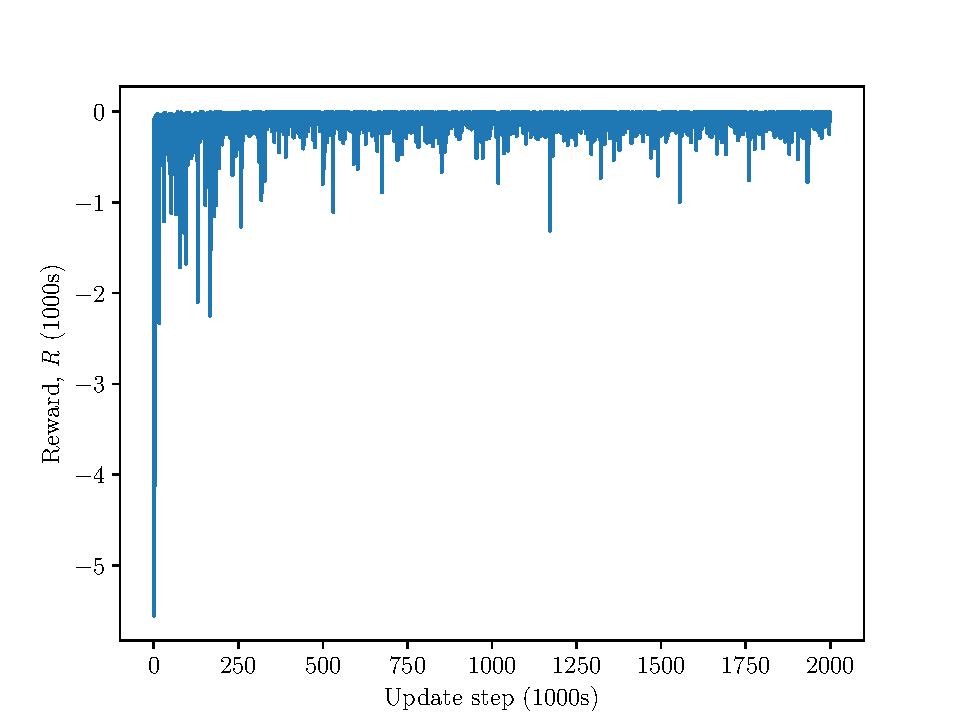
\includegraphics[width=0.66\textwidth]{images/ch4/loss_curve.pdf}
    \caption{Loss curve of the agent during training.}
    \label{fig:loss_curve}
\end{figure}

\subsection{Step 4: Online calibration}

The agent was then applied onto the real process to track pressure set-points of 35 and 5.  The output pressure trajectory of the Mechatronix is shown in \ref{fig:system1_highsp} and \ref{fig:system1_lowsp}. Performance-wise, the MSE was $14.2$ and $15.5$ for set-points 35 and 5, respectively. To ensure a fair comparison, both cases started with initial pressures approximately 5.5 kPa above the desired set-point. In this simple set-up, the agent behaves much like a PID where the RL maps tracking errors to changes in input and is linear in nature. Unfortunately, such a set-up only works well locally for non-linear systems. Moreover, the performance decreases significantly as the agent ponders away from the linear region, as shown in Figure \ref{fig:system1_lowsp}. In this experiment, the agent's performance is significantly better when tracking $P=35$ because the training set-points were heavily biased towards $P=35$.  From Figure \ref{fig:04model_fit}, it can be seen quite obviously that the controller gain changes significantly at lower pressures, resulting in the optimal policy for the higher pressure range being completely sub-optimal at lower pressures. Furthermore, the large off-set seen in these trajectories are caused by the discretization error; there exists no action $\Delta u \in \mathcal{U}$ that can obtain exactly $P = 35 \; or \; 5 \; kPa$. To overcome this, one option is to discretize the action space more finely, but this will unavoidably the increase the training time and space complexity required by the agent (perhaps by a massive margin).  A simpler way will be introduced in the latter half of this example.

\begin{figure}[H]
     \centering
     \begin{subfigure}{0.49\textwidth}
         \centering
         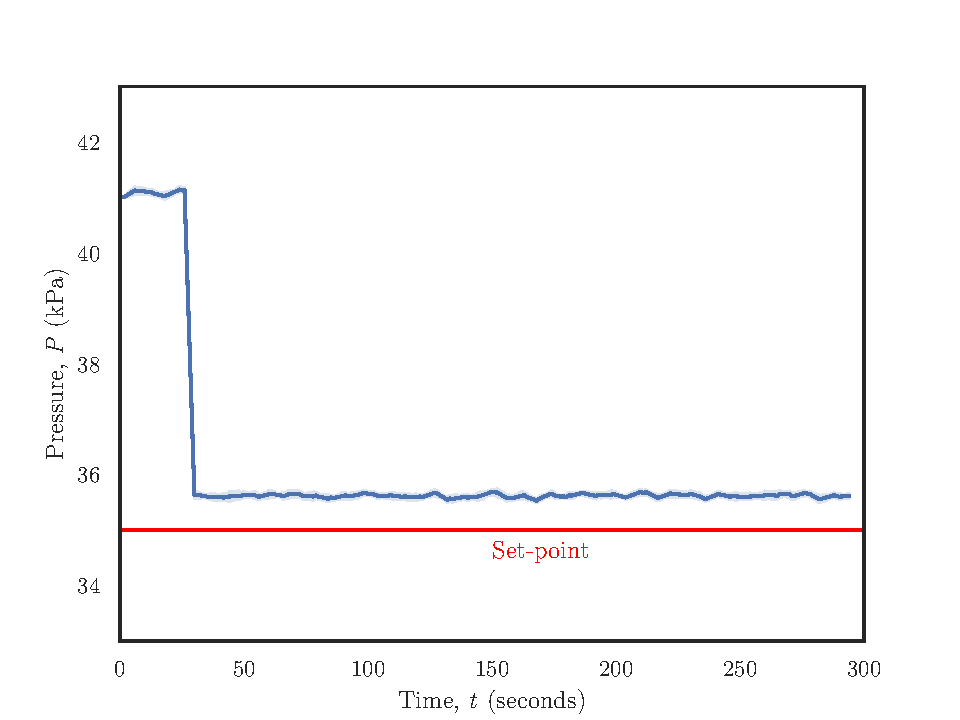
\includegraphics[width=\textwidth]{images/ch4/35SP_normal.pdf}
         \caption{Tracking $P_{sp} = 35 \; kPa$}
         \label{fig:system1_highsp}
     \end{subfigure}
     \hfill
     \begin{subfigure}{0.49\textwidth}
         \centering
         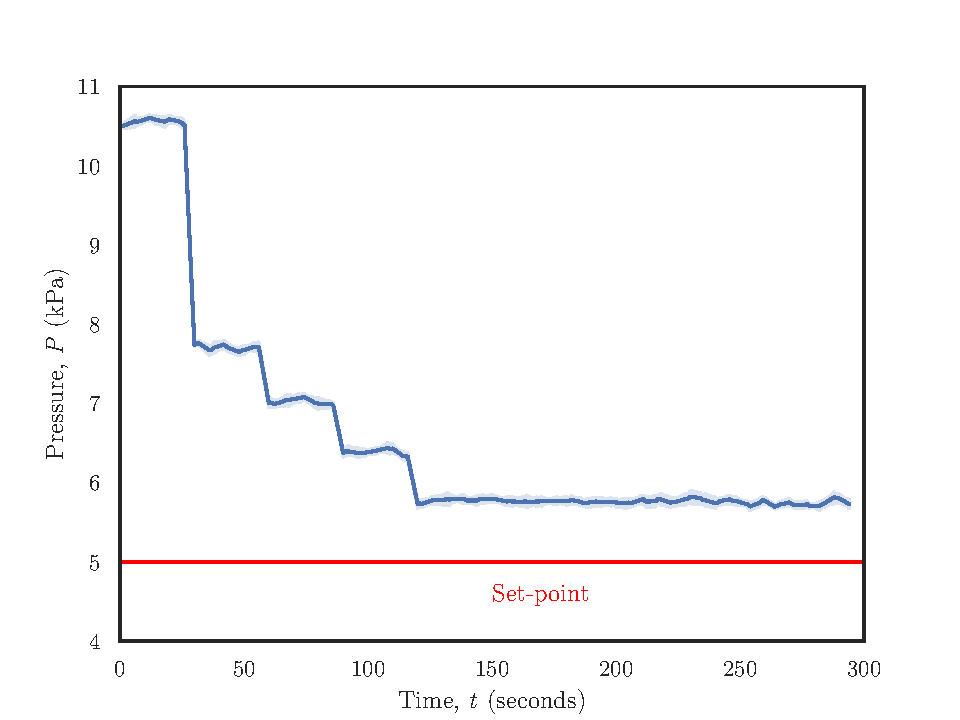
\includegraphics[width=\textwidth]{images/ch4/5SP_normal.pdf}
         \caption{Tracking $P_{sp} = 5 \; kPa$}
         \label{fig:system1_lowsp}
     \end{subfigure}
     \caption{Pressure trajectory of the Mechatronix experiment.  Solid line represents the average of 10 runs to ensure reproducability. Shaded area correspond to one standard deviation.}
\end{figure}

\subsection{Extension to Non-linear Systems}
A simple, cost effective way for the agent's capabilities to extend to non-linear systems is to model the system using a linear parameter-varying model as shown in Figure \ref{fig:model_fit_approx}. This way, each sub-piece of the model is linear, allowing even linear control laws to be optimal.  To create a Markovian setting, the agent will receive this information through a \textit{second state} given by:
\[
    x^{(2)}= 
\begin{cases}
    1,              & \text{if } P  \leq 10 \\
    2,              & \text{if } 10 <  P  \leq 20 \\
    3,              & \text{if } 20 <  P  \leq 30 \\
    4,              & \text{if } 30 <  P  \leq 50 \\
    5,              & P > 50 \\
\end{cases}
\]
The new state space for the agent is given by:
\begin{equation}
    x = [(-20, 1), (-20, 2), (-20, 3), ..., (-19, 1), ..., (20, 5)]_{1 \times 205}
\end{equation}
where the first value denotes the error and the second value correspond to the region the agent is currently in. Here, the $Q$-matrix will be initialized as $0_{(41 \cdot 5) \times 3}$ to accommodate for the second state. Intuitively, the agent now observes both the magnitude and the context of the incurred tracking error; intrinsically, allowing the agent to change its policy depending on the region it is currently in.

\begin{figure}[H]
    \centering
    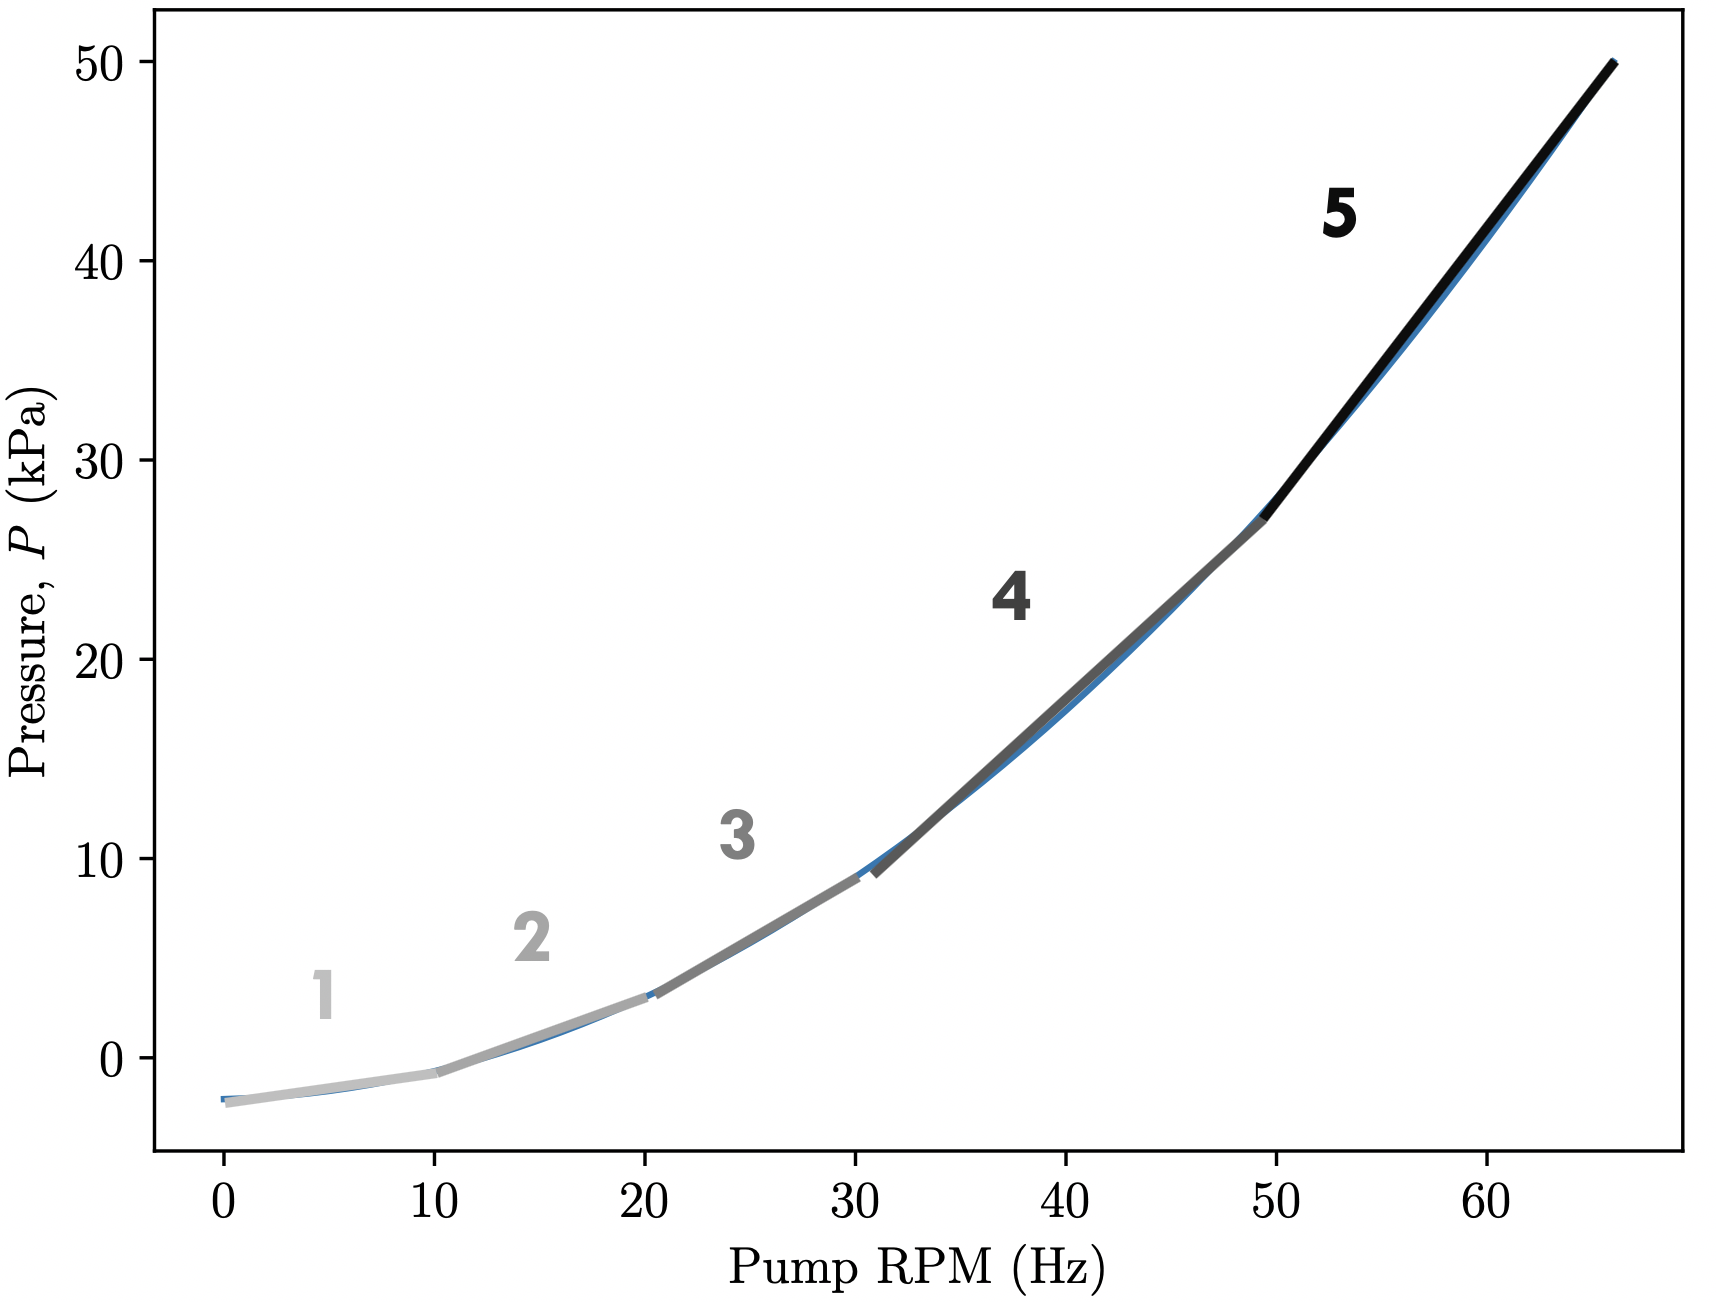
\includegraphics[width=0.62\textwidth]{images/ch4/model_fit_approx.jpeg}
    \caption{Approximating the non-linear Mechatronix system.}
    \label{fig:model_fit_approx}
\end{figure}

The new agent was implemented onto Mechatronix after 2,000,000 time steps of training.  The new agent's output pressure trajectories for tracking $P=35$ and 5 are shown in Figures \ref{fig:system1_highsp2} and \ref{fig:system1_lowsp2}.  Performance-wise, the agent achieved  MSEs of 14.2 and 12.5 for the higher and lower set-point; a massive improvement for the lower set-point.  Nevertheless, the offset still exists.

\begin{figure}[H]
     \centering
     \begin{subfigure}{0.49\textwidth}
         \centering
         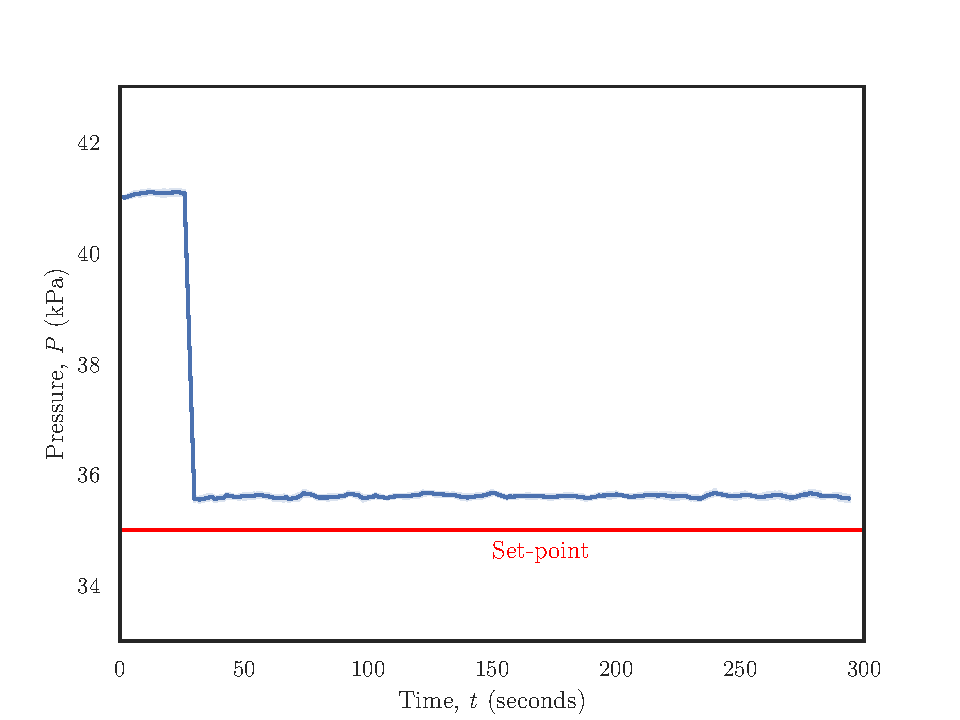
\includegraphics[width=\textwidth]{images/ch4/35SP_2state.pdf}
         \caption{Tracking $P_{sp} = 35 \; kPa$}
         \label{fig:system1_highsp2}
     \end{subfigure}
     \hfill
     \begin{subfigure}{0.49\textwidth}
         \centering
         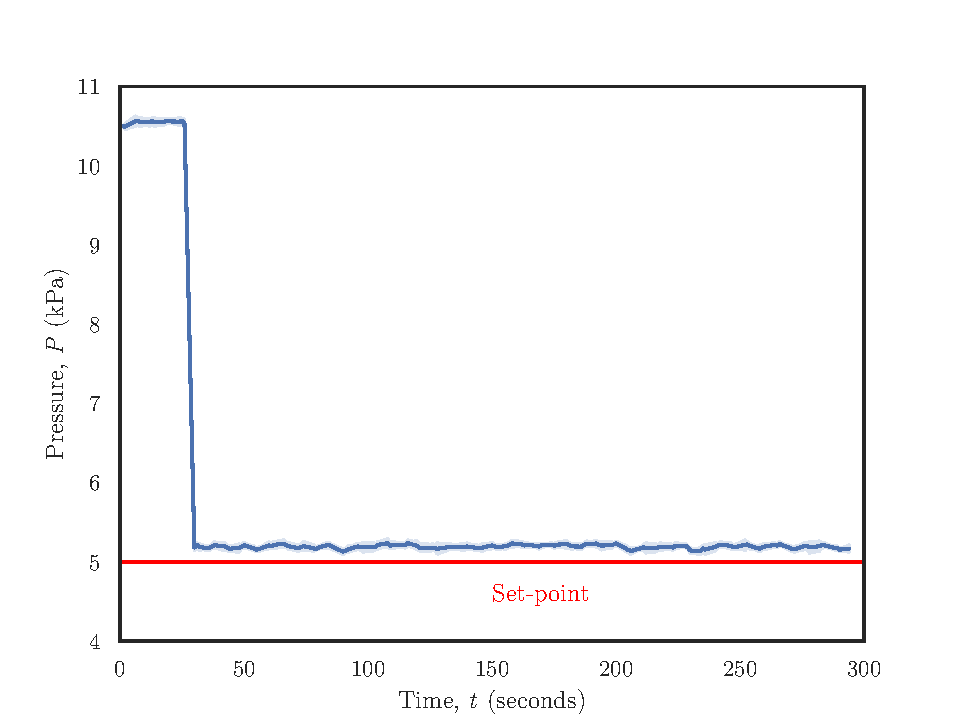
\includegraphics[width=\textwidth]{images/ch4/5SP_2state.pdf}
         \caption{Tracking $P_{sp} = 5 \; kPa$}
         \label{fig:system1_lowsp2}
     \end{subfigure}
     \caption{Pressure trajectory using the non-linear agent. Solid line represents the average of 10 runs to ensure reproducability. Shaded area correspond to one standard deviation.}
\end{figure}



\subsection{Extension to continuous states and actions}
Because the non-linear system was approximated using a LPV model, the control law for the system should be always linear. Because of this, linear interpolation can be used to find the optimal control action using \cite{interpolation}:
\begin{equation}
    u = u_{low} + (x - x_{low})\frac{u_{high} - u_{low}}{x_{high} - x_{low}}
    \label{eq:interpolation}
\end{equation}
where $x$ is the actual tracking error; typically, the exact value of $x$ is not included in the discretized state space $\mathcal{X}$.  Instead, $x$ is typically between $x_{high}$ and $x_{low}$, where $x_{high}$ and $x_{low}$ correspond to the state that is higher and lower than $x$, respectively.  For example, if the discretized state space is given as $x = [0, -5, -10]$ and the current state is -3, $x_{high}$ and $x_{low}$ would be 0 and -5, respectively.  Similarily, $u_{high}$ and $u_{low}$ are the greedy actions for $x_{high}$ and $x_{low}$, respectively. For example, given the action space $u=[-5, 0, 5]$ and $Q-$matrix:

    $$ Q(x, u) = \left(\begin{matrix}   -5  &  2  & 1 \\\
                                        4 & 1 & -2 \\
                                        -2 & 0 & 3 \end{matrix}\right), $$
                                        
$u_{high}$ and $u_{low}$ are 0 and -5 (actions corresponding to the index of the highest $Q$-value), respectively. Moreover, the optimal action for $x = -3$ would be:
$$u = -5 + (-3 + 5) \frac{0 + 5}{0 + 5}$$
$$u = -3$$

With the addition of interpolation action selection, the 2-state RL agent (without re-training the agent) achieved pressure trajectories shown in Figures \ref{fig:system1_highsp3} and \ref{fig:system1_lowsp3} with MSEs of 13.6 and 11.7, respectively. Additionally, it can be seen that the off-set is completely eliminated.

\begin{figure}[H]
     \centering
     \begin{subfigure}{0.49\textwidth}
         \centering
         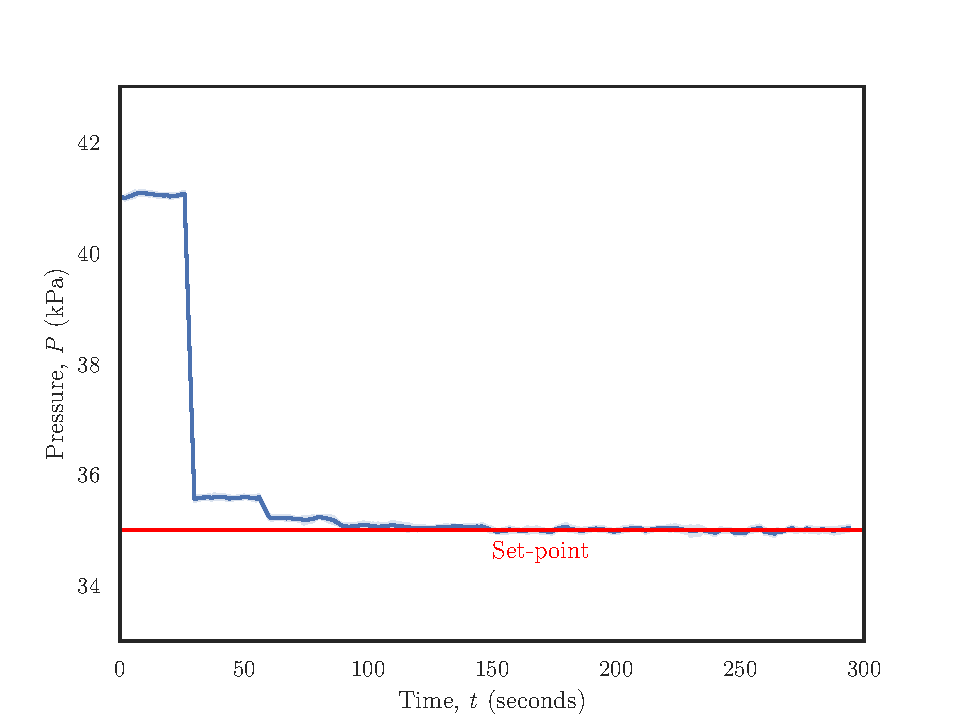
\includegraphics[width=\textwidth]{images/ch4/35SP_interpolation.pdf}
         \caption{Tracking $P_{sp} = 35 \; kPa$}
         \label{fig:system1_highsp3}
     \end{subfigure}
     \hfill
     \begin{subfigure}{0.49\textwidth}
         \centering
         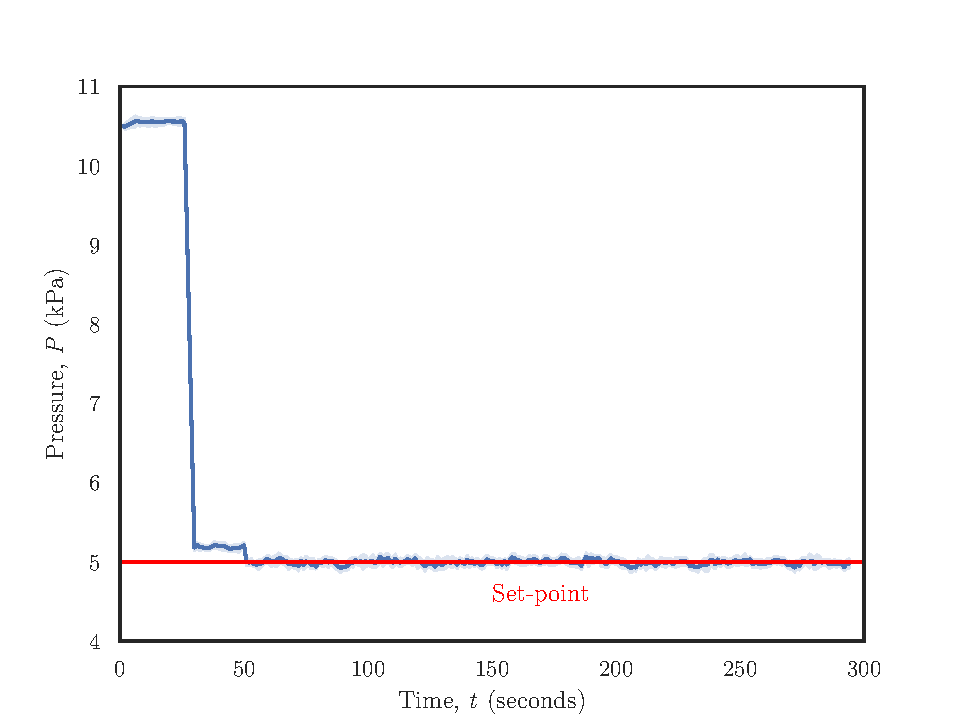
\includegraphics[width=\textwidth]{images/ch4/5SP_interpolation.pdf}
         \caption{Tracking $P_{sp} = 5 \; kPa$}
         \label{fig:system1_lowsp3}
     \end{subfigure}
     \caption{Pressure trajectory of the non-linear agent using interpolation action selection. Solid line represents the average of 10 runs to ensure reproducability. Shaded area correspond to one standard deviation.}
\end{figure}

The RL methods introduced in this section along with their respective characteristics are summarized in Table \ref{tab:system1_info}. Throughout this tutorial, a simple RL agent was implemented onto an industrial VFD system. It was shown that the vanilla algorithm was unable to handle neither non-linear systems or achieve off-set free control; therefore, simple, implementable techniques that extended the agent's ability to non-linear systems and for off-set free control were introduced. Each state trajectory in this study was replicated on the live systems 10 times to ensure reproducability; the standard deviation for every algorithm was very narrow, representing highly reproducible results (indirectly, less risk).

\begin{table}[H]
\caption{A comparison between RL, MPC in literature, and industrial MPC software.}
\label{tab:system1_info}
\centering
{\scriptsize
\begin{tabular}{c|c|c|c}
 & \textbf{Normal $Q$-learning}	& \textbf{2-state $Q$-learning} & \textbf{2-state interpolated $Q$-learning}\\
 \hline
MSE (High/Low SP)   & 14.2 \& 15.5	& 14.2 \& 12.5   &  13.6 \& 11.7 \\
Offset		& Yes			&  Yes   &  No \\
Non-linear		& No			& Yes   &  Yes \\
\end{tabular}}
\end{table}

In the implementation above, the agent only provided the input for the \textit{immediate} future. A concept very similar to MPC where only the next input is used; however, MPC is considered receding horizon control, where an input trajectory for future steps is also calculated.  Using this trajectory, MPC is viable for short horizon open-loop control.  Comparatively, RL can also conduct receding horizon control. Such RL methods typically employ a model of the system and are called planning methods.  In receding horizon RL, the agent still only outputs the immediate control action; however, it then uses the model to identify the next state and its corresponding optimal control action. The cycle continues until the set control horizon is met.  Additionally, like MPC, the trajectory is heavily inaccurate for long control horizons.

The example shown here is simple, has a pre-set sampling time and does not consider transition dynamics or unobservable states. For systems containing dynamic transition times and to consider systems dynamics, semi-MDPs must be used.  The semi-MDP variant of Q-learning algorithm is \cite{continuous_rl_ref14}:
\begin{equation}
    Q(x, u) \leftarrow Q(x, u) + \alpha \left[\frac{1 - e^{-\beta \tau}}{\beta}r(x, x_{t+1}, u) + e^{-\beta \tau} \max_{u_{t+1}}Q(x_{t+1}, u_{t+1}) - Q(x, u) \right]
\end{equation}
where $r(x_t, x_{t+1}, u)$ is the reward rate and is provided in Equation \ref{eq:reward_rate}. For systems with unmeasurable states, concepts of POMDPs provided in Chapter 1 should be used.

\section{Control of Wastewater Treatment Plant}


















\section{Optimality Evaluation of Reinforcement Learning}
UCB tabular $Q$-learning suffers from discretized states and actions and the curse of dimensionality.  To overcome such issues, deep RL will be explored.  More specifically, this section uses the deep deterministic policy gradient (DDPG) algorithm introduced in Chapter 1. DDPG offers several advantages and disadvantages compared to tabular $Q$-learning.  The advantages are that it can handle continuous states and perform continuous actions. Furthermore, the scalability of the algorithm is greatly enhanced because deep function approximators are used to map states to actions, rather than a $Q$-table. However, these advantages come with some disadvantages.  First and foremost, DDPG is a black box approach and employs four deep neural networks to perform function approximation; therefore, explicitly identifying the control policy for DDPG is nearly impossible. Secondly, the function approximations cause small perturbations in control.  That is, the control outputs can sometimes contain small "jitters" (given an ideal output of 1, DDPG may output values between 0.995 - 1.005).  Intuitively, this is caused by the generality of the algorithm and can be related to humans.  Humans possess perhaps one of the most general intelligence available, yet we are not even capable of drawing a straight line. DDPG follows a similar idea; the algorithm is so general that it sometimes struggle with highly precise actions. For advanced details regarding DDPG, see \cite{ddpg}.  

The objective of this section is to \textbf{explore the optimality} of RL and how closely it can approach the optimal solution (assuming MPC provides the optimal solution when given a perfect process model).  Here, four different control strategies will be applied onto simple SISO, SIMO, MISO, and MIMO systems. The four strategies are shown in Table \ref{tab:04control_and_cost}.

\begin{table}[H]
\caption{Different control strategies to be compared.}
\centering
\begin{tabular}{c|c}
\textbf{Control Algorithm} & \textbf{Reward Function}\\
\hline
MPC		                & MPC cost function		 \\
Tabular $Q$-learning    & MPC cost function		 \\
DDPG	                & MPC cost function		 \\
DDPG         	        & Custom RL reward function	
\label{tab:04control_and_cost}
\end{tabular}
\end{table}

From Table \ref{tab:04control_and_cost}, the MPC cost function is given as:
\begin{equation}
    J = \sum\limits^{N}_{i = 1} x_i^TQ_{mpc}x_i + \sum\limits^N_{i=1}u_i^TR_{mpc}u_i
    \label{eq:04mpc_cost}
\end{equation}
where:
$$x_i = x_t - x_{ss}$$ 
$$u_i = u_t - u_{ss}$$ 
and the custom RL reward function is:
\[
    reward = 
\begin{cases}
    15 - (x_t - x_{sp}) \times 15,              & \text{if } x_i \leq 1 \\
    x_i^2 + u_i^2,              & otherwise \\
    \label{eq:04rl_cost}
\end{cases}
\]

\subsection{Single-Input Single-Output System}
First, a SISO system will be used to benchmark RL against MPC.  The system is given by:
\begin{equation}
\dfrac{dx}{dt} = -4x + u
\end{equation}
\noindent
In the s-domain, the system equation is:
\begin{equation}
Y(s) = \dfrac{1}{s + 4}
\end{equation}
The system is stable with one pole at -4.  Initially, the system is at steady state with:
$$x_0 = 0.5$$
$$u_0 = 1.0$$
The steady-state state and input, $x_{ss}$ and $u_{ss}$, are:
$$x_{ss} = 5.0$$ 
$$u_{ss} = 10.0$$
Here, MPC used a prediction and control horizon of 20, with $Q_{mpc}$ and $R_{mpc}$ as 0.1 and 0.1, respectively.  The RL hyper parameters are given in Tables \ref{tab:04tab_rl} and \ref{tab:04deep_rl}

\begin{table}[H]
\caption{Tabular RL hyper parameters for the SISO system.}
\label{tab:04tab_rl}
\centering
\begin{tabular}{c|c}
\textbf{Hyper Parameter}     & \textbf{Value}  \\
\hline
States, $x$	             	& $[0, 0.18, ..., 8]_{1 \times 45} $		 \\
Actions, $u$               & $[5, 5.22, ..., 15]_{1 \times 45}$		\\
Reward, $r$	               & Equation \ref{eq:04mpc_cost}		\\
Learning rate, $\alpha$		& [0.001, 0.7]		 \\
Discount factor, $\gamma$      	& 0.95  \\
Exploratory factor, $\epsilon$             & [0.1, 1]  \\
Evaluation time                 & 1 second \\
System representation           & FOMDP \\
\end{tabular}
\end{table}

\begin{table}[H]
\caption{DDPG hyper parameters for the SISO system.}
\label{tab:04deep_rl}
\centering
\begin{tabular}{c|c}
\textbf{Hyper Parameter}     & \textbf{Value}  \\
\hline
Actor network size	             & 3 layers: 50, 40, 40 neurons		 \\
Actor learning rate              & 0.0001		\\
Critic network size	             & 3 layers: 40, 30, 30 neurons		\\
Critic learning rate       		 & 0.001		 \\
Reward, $r$	                     & Equation \ref{eq:04mpc_cost}	or Equation \ref{eq:04rl_cost}	\\
Discount factor, $\gamma$      	& 0.95  \\
Evaluation time                 & 1 second \\
System representation           & FOMDP \\
\end{tabular}
\end{table}

Figure \ref{fig:04SISOcomp} shows the input and state trajectories of the four control algorithms. The total cost of each trajectory (all calculated using Equation \ref{eq:04mpc_cost}) are shown in Table \ref{tab:04SISOCost}. Ultimately, RL actually \textit{surpassed} the performance of MPC in this case, even when equipped with a perfect process model. Comparing the trajectories, it can be seen that RL started with aggressive inputs, but reduced the magnitude thereafter.  On the other hand, MPC started with a smaller initial inputs, and gradually increased it along the trajectory. Deep RL had the "poorest" cost performance; it achieved the state set-point, but incurred large losses with its aggressive inputs. In theory, MPCs using a perfect process model will output the optimal solution.  In this case, one source of error could be the discount factor in RL that is not present in MPC. Typically, a discount factor of 0.95 denotes a 20 prediction horizon \cite{deeplearning_course}; however, these are not exactly equivalent. Nevertheless, this small scale study demonstrates that RL can actually surpass MPC even when the cost functions are \textit{nearly} identical.  

\begin{figure}[H]
    \centering
    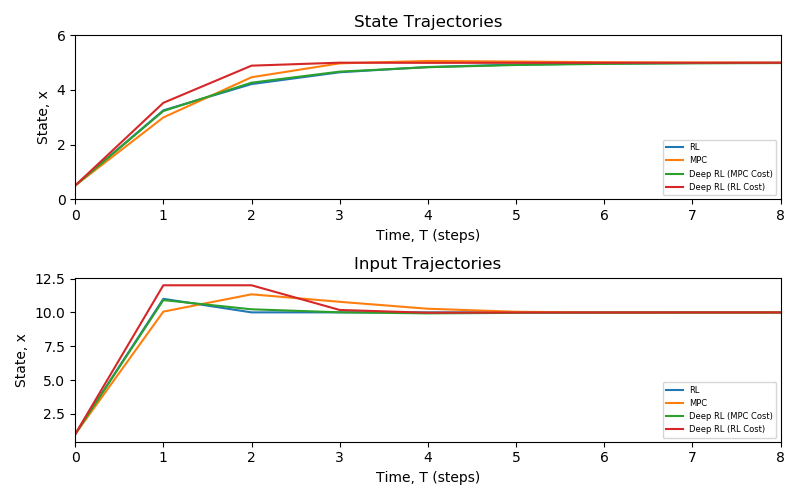
\includegraphics[width=0.9\textwidth]{images/ch4/States_and_Inputs_SISO2.png}
    \caption{Input and state trajectories of the four control strategies on the SISO system.}
    \label{fig:04SISOcomp}
\end{figure}

\begin{table}[H]
\caption{Controller cost for the input and state trajectories on the SISO system.}
\label{tab:04SISOCost}
\centering
\begin{tabular}{c|c|c|c}
\textbf{MPC} & \textbf{Tabular RL} & \textbf{Deep RL with MPC cost}& \textbf{Deep RL with RL cost} \\
\hline
5.56	     & 4.55	               & 4.27                         & 6.19	 \\
\end{tabular}
\end{table}







\subsection{Multiple-Input Multiple-Output System}
The above study was repeated for a simple MIMO system described by:
\begin{flalign}
\dfrac{dx_1}{dt} &= -3x_1 - 2x_2 + 4u_1 \\
\dfrac{dx_2}{dt} &= -3x_2 + 2u_2
\end{flalign}
In the s-domain, the system equations are:
\begin{align}
Y_1(s) = \dfrac{4}{(s+3)^2} \\
Y_2(s) = \dfrac{2}{(s+3)^2}
\end{align}
The system is critical damped and stable (i.e., two identical poles at -3). Initially, the system is at steady state with:
\begin{align}
x_{0} = \begin{bmatrix}
           1.3 \\
           4.0
         \end{bmatrix}
u_{0} = \begin{bmatrix}
           3.0 \\
           6.0
         \end{bmatrix}
\end{align}
The steady-state states and inputs, $x_{ss}$ and $u_{ss}$ are:
\begin{center}
$x_{ss} = \begin{bmatrix}
           3.6 \\
           4.7
         \end{bmatrix}$ \\
\vspace{3mm}
$u_{ss} = \begin{bmatrix}
           5.0 \\
           7.0
         \end{bmatrix}$ \\
\end{center}

The MPC for this system also has a prediction and control horizon of 20.  The $Q$ and $R$ matrices are given by:
$$Q = \begin{bmatrix}
	1 & 0 \\
	0 & 1
\end{bmatrix}$$

$$R = \begin{bmatrix}
	1   & 0 \\
	0   & 1
\end{bmatrix}$$

The RL hyper parameters for the MIMO system is given in Tables \ref{tab:04tab_rl_mimo} and \ref{tab:04deep_rl_mimo}.
\begin{table}[H]
\caption{Tabular RL hyper parameters for the MIMO system.}
\label{tab:04tab_rl_mimo}
\centering
\begin{tabular}{c|c}
\textbf{Hyper Parameter}     & \textbf{Value}  \\
\hline
States, $x$	             	& $x_1 = [0, 0.5, ..., 6]_{1 \times 13} $		 \\
        	             	& $x_2 = [2, 2.5, ..., 6]_{1 \times 9} $		 \\
Actions, $u$                & $u_1 = [1, 2, ..., 7]_{1 \times 7}$	         \\
                            & $u_2 = [4, 5, ..., 9]_{1 \times 6}$		\\
Reward, $r$	                & Equation \ref{eq:04mpc_cost}		\\
Learning rate, $\alpha$		& [0.001, 0.5]		 \\
Discount factor, $\gamma$      	& 0.95  \\
Exploratory factor, $\epsilon$             & [0.1, 1]  \\
Evaluation time                 & 1 second \\
System representation           & FOMDP \\
\end{tabular}
\end{table}

\begin{table}[H]
\caption{DDPG hyper parameters for the MIMO system (identical to the SISO system).}
\label{tab:04deep_rl_mimo}
\centering
\begin{tabular}{c|c}
\textbf{Hyper Parameter}     & \textbf{Value}  \\
\hline
Actor network size	             & 3 layers: 50, 40, 40 neurons		 \\
Actor learning rate              & 0.0001		\\
Critic network size	             & 3 layers: 40, 30, 30 neurons		\\
Critic learning rate       		 & 0.001		 \\
Reward, $r$	                     & Equation \ref{eq:04mpc_cost}	or Equation \ref{eq:04rl_cost}	\\
Discount factor, $\gamma$      	& 0.95  \\
Evaluation time                 & 1 second \\
System representation           & FOMDP \\
\end{tabular}
\end{table}

Figure \ref{fig:04MIMOcomp} shows the input and state trajectories of the MIMO system using the four control methods.  The total cost of each trajectory (again calculated using Equation \ref{eq:04mpc_cost}) is shown in Table \ref{tab:04MIMOCost}. Here, MPC performed the best while the two deep RL methods performed the worst. Furthermore, tabular RL's performance was nearly identical to MPC. Comparing the trajectories, the deep RL tends to favour $x_2$ and made large actions in $u_2$ while MPC and tabular RL instead focused on $x_1$.  It is difficult to identify exactly why deep RL favored $x_2$.
Perhaps it was because $x_2$ was only a function of itself and $u_2$, but the exact reason is unknown.
\begin{figure}[H]
    \centering
    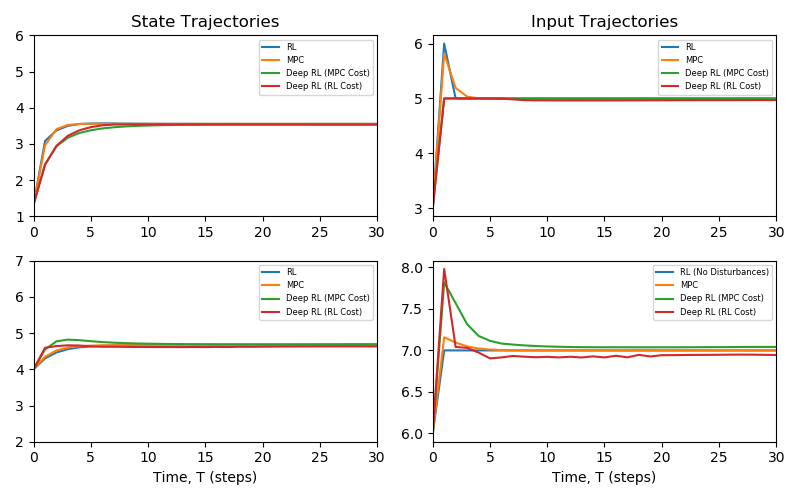
\includegraphics[width=0.9\textwidth]{images/ch4/State_and_Input_MIMO3.png}
    \caption{Input and state trajectories of the four control strategies on the MIMO system. The top figures denote $x_1$ and $u_1$.  The bottom figures denote $x_2$ and $u_2$.}
    \label{fig:04MIMOcomp}
\end{figure}

\begin{table}[H]
\caption{Controller cost for the input and state trajectories on the MIMO system.}
\label{tab:04MIMOCost}
\centering
\begin{tabular}{c|c|c|c}
\textbf{MPC} & \textbf{Tabular RL} & \textbf{Deep RL with MPC cost}& \textbf{Deep RL with RL cost} \\
\hline
0.86	     & 0.95	               & 2.33                         & 2.59	 \\
\end{tabular}
\end{table}

\subsection{Discounted Stage Cost for MPC}
To enhance the comparability of the two methods, MPC was changed to have an infinite horizon; however, the cost function would be discounted at each successive state.  The new MPC cost function is given as:
\begin{equation}
    J = \sum^{N}_{i = 1} \gamma^i[x^TQx + u^TRu]
    \label{eq:04disc_mpc}
\end{equation}

Using this new cost function, the previous comparisons along with new SIMO and MISO systems were used to compare the four control strategies.  The new state and input trajectories of the SISO, SIMO, MISO, and MIMO systems using the four control strategies are shown in Figures \ref{fig:04SISO_disc}, \ref{fig:04SIMO_disc}, \ref{fig:04MISO_disc}, and \ref{fig:04MIMO_disc}, respectively.  The system descriptions and the costs are provided in Table \ref{tab:04allsys}.  Note that the deep RL using the custom RL cost was omitted here because it under-performed in all previous scenarios.  It can be seen that after discounting was introduced into the MPC cost function, all trajectories look nearly identical with only slight differences.  MPC was able to achieve the lowest cost (theoretically sound); however, RL and deep RL both achieved very comparable results through self-play alone!  From these plots, it can be concluded that RL does indeed approach the optimality of MPC, although cannot achieve exactly the optimal results.

\begin{figure}[H]
    \centering
    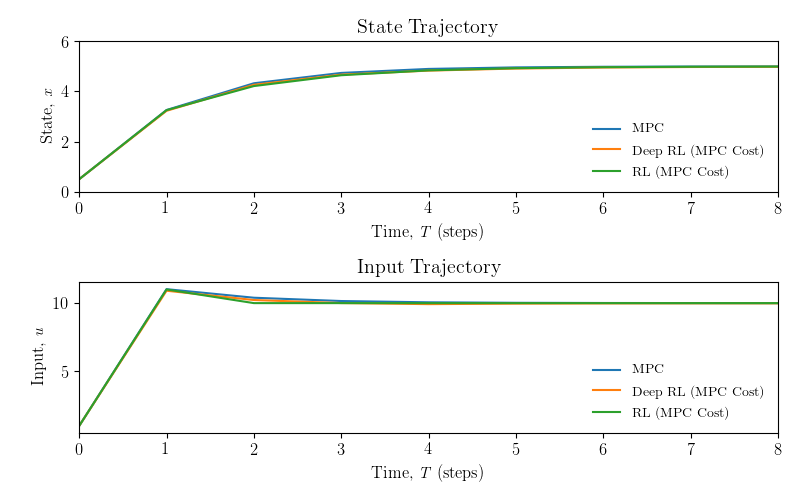
\includegraphics[width=0.9\textwidth]{images/ch4/State_and_Input.png}
    \caption{Input and state trajectories of the four control strategies on the SISO system.  MPC cost is calculated using Equation \ref{eq:04disc_mpc}.}
    \label{fig:04SISO_disc}
\end{figure}

\begin{figure}[H]
    \centering
    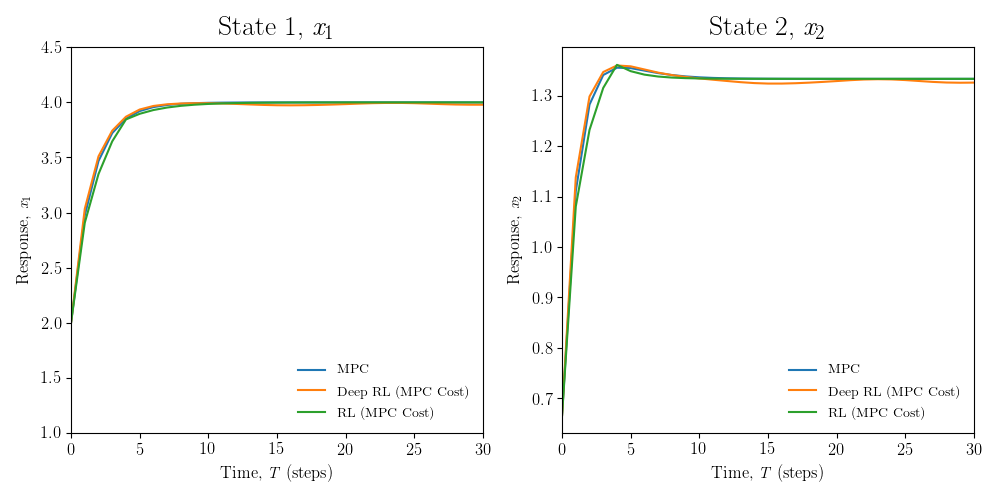
\includegraphics[width=0.9\textwidth]{images/ch4/State_SIMO.png}
    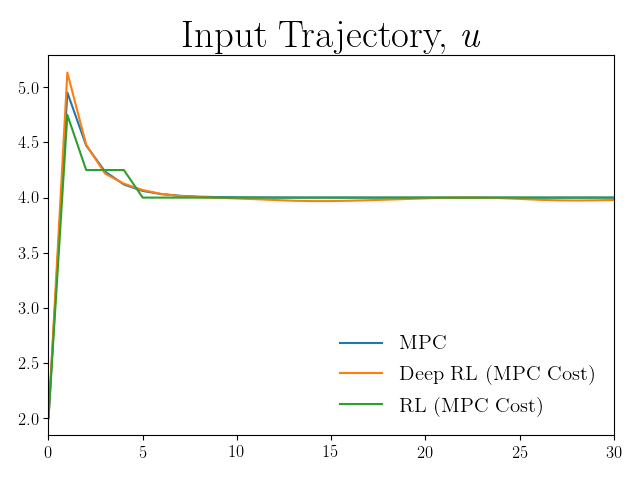
\includegraphics[width=0.52\textwidth]{images/ch4/Input_SIMO.png}
    \caption{Input and state trajectories of the four control strategies on the SIMO system.  MPC cost is calculated using Equation \ref{eq:04disc_mpc}.}
    \label{fig:04SIMO_disc}
\end{figure}

\begin{figure}[H]
    \centering
    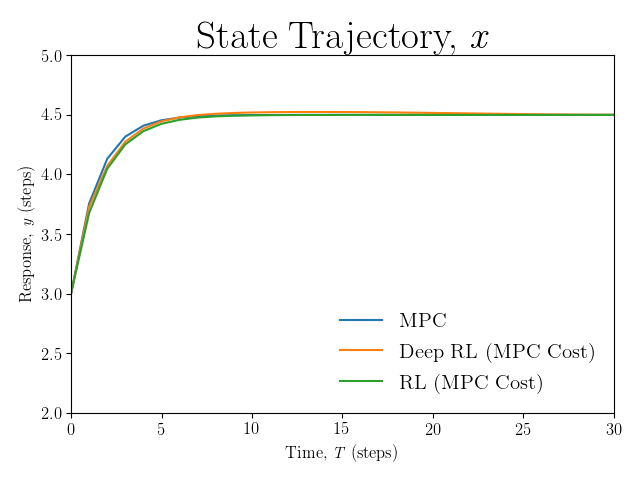
\includegraphics[width=0.52\textwidth]{images/ch4/State_MISO.png}
    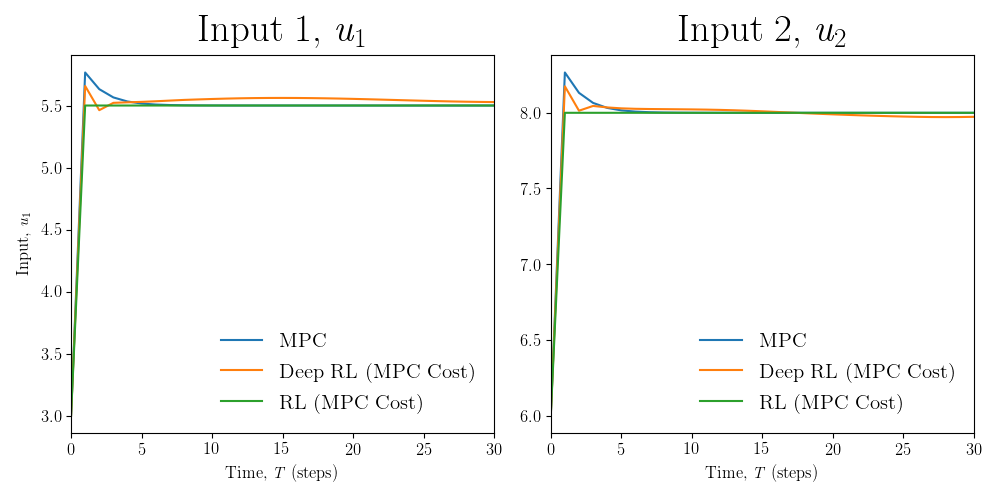
\includegraphics[width=0.9\textwidth]{images/ch4/Input_MISO.png}
    \caption{Input and state trajectories of the four control strategies on the MISO system.  MPC cost is calculated using Equation \ref{eq:04disc_mpc}.}
    \label{fig:04MISO_disc}
\end{figure}

\begin{figure}[H]
    \centering
    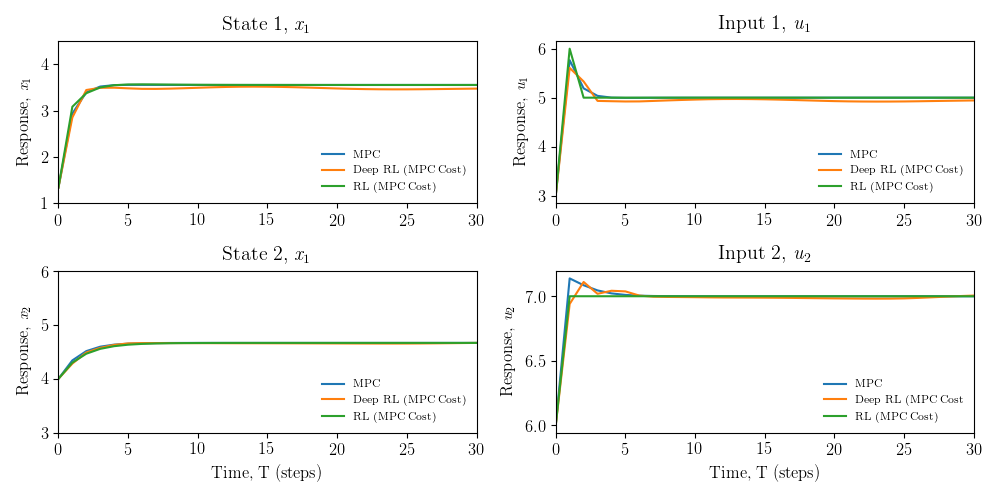
\includegraphics[width=0.9\textwidth]{images/ch4/State_and_Input_MIMO.png}
    \caption{Input and state trajectories of the four control strategies on the MIMO system. MPC cost is calculated using Equation \ref{eq:04disc_mpc}}
    \label{fig:04MIMO_disc}
\end{figure}

\begin{table}[H]
\caption{Controller cost for the input and state trajectories on the MIMO system.}
\label{tab:04allsys}
\centering
{\tiny
{\setstretch{2.8}
\begin{tabular}{c|c|c|c|c}
           &  \textbf{SISO} & \textbf{SIMO} & \textbf{MISO}& \textbf{MIMO} \\
\hline
System Equation & $\dfrac{dx}{dt} = -4x + u$ & $\dfrac{dx_1}{dt} = -2x_1 + u$	     & $\dfrac{dx}{dt} = -3x + u_1 + u_2$         & $\dfrac{dx_1}{dt} = -3x_1 - 2x_2 + 4u_1$	 \\
&  & $\dfrac{dx_2}{dt} = -3x_2 + u$	     &         & $\dfrac{dx_2}{dt} = -3x_2 + 2u_2$  \\ \hline


Initial States  & $x_0 = 0.5$ & $x_0 = [2.0, 0.7]$	  & $x_0 = 3.0$         & $x_{ss} = [1.3, 4.0]$	 \\
                & $u_0 = 1.0$ & $u_0 = 2.0$		               & $u_0 = [3.0, 6.0]$        & $u_{ss} = [3.0, 6.0]$	 \\ \hline


Steady States   & $x_{ss} = 5.0$ & $x_{ss} = [4.0, 4.3]$	 & $x_{ss} = 4.5$         & $x_{ss} = [3.6, 4.7]$	 \\
                & $u_{ss} = 10.0$ & $u_{ss} = 4.0$	         & $u_{ss} = [5.5, 8.0$   & $u_{ss} = [5.0, 7.0]$		 \\ \hline


MPC Cost            & 4.18	     & 2.1	               & 0.83         & 0.87	 \\
Tabular RL Cost     & 4.33	     & 2.2	               & 0.97         & 0.95	 \\
Deep RL Cost        & 4.32	     & 2.1	               & 0.89         & 1.14	 \\
\end{tabular}}}
\end{table}

\subsection{Comparison of RL and MPC on a CSTR}
All previous systems were applied onto arbitrary linear systems that do not exist in the real world. Here, a non-linear CSTR system will be used to evaluate the optimality of each control strategy. The CSTR is given by the following differential equations:
















\section{A Study on Interpolated RL}


\section{Comparison of Optimal Control Frameworks}
The control framework of a typical process was first introduced in Chapter 1, and is shown again here in Figure \ref{fig:rto_mpc_pid2}. As a brief refresher: RTO evaluates seldomly (hourly basis) and is used to find the optimal steady states with accordance to a desired performance metric \cite{rto}. These optimal steady states are then passed onto the MPC layer, where the optimal input trajectories are identified.  A typical MPC objective function is:
\begin{equation}
    J = \sum\limits_{i = 1}^{H}x_i^TQ_{mpc}x_i + u_i^TR_{mpc}u_i
    \label{eq:mpc}
\end{equation}
due to its convexity \cite{mpc}. In recent advanced control literature, researchers intertwined the concepts of RTO and MPC into one unifying algorithm that is now known as economic model predictive control (EMPC) \cite{empc1, empc2}. Here, the objective function of EMPC explicitly contains the economic objectives of the process.

\begin{figure}[H]
    \centering
    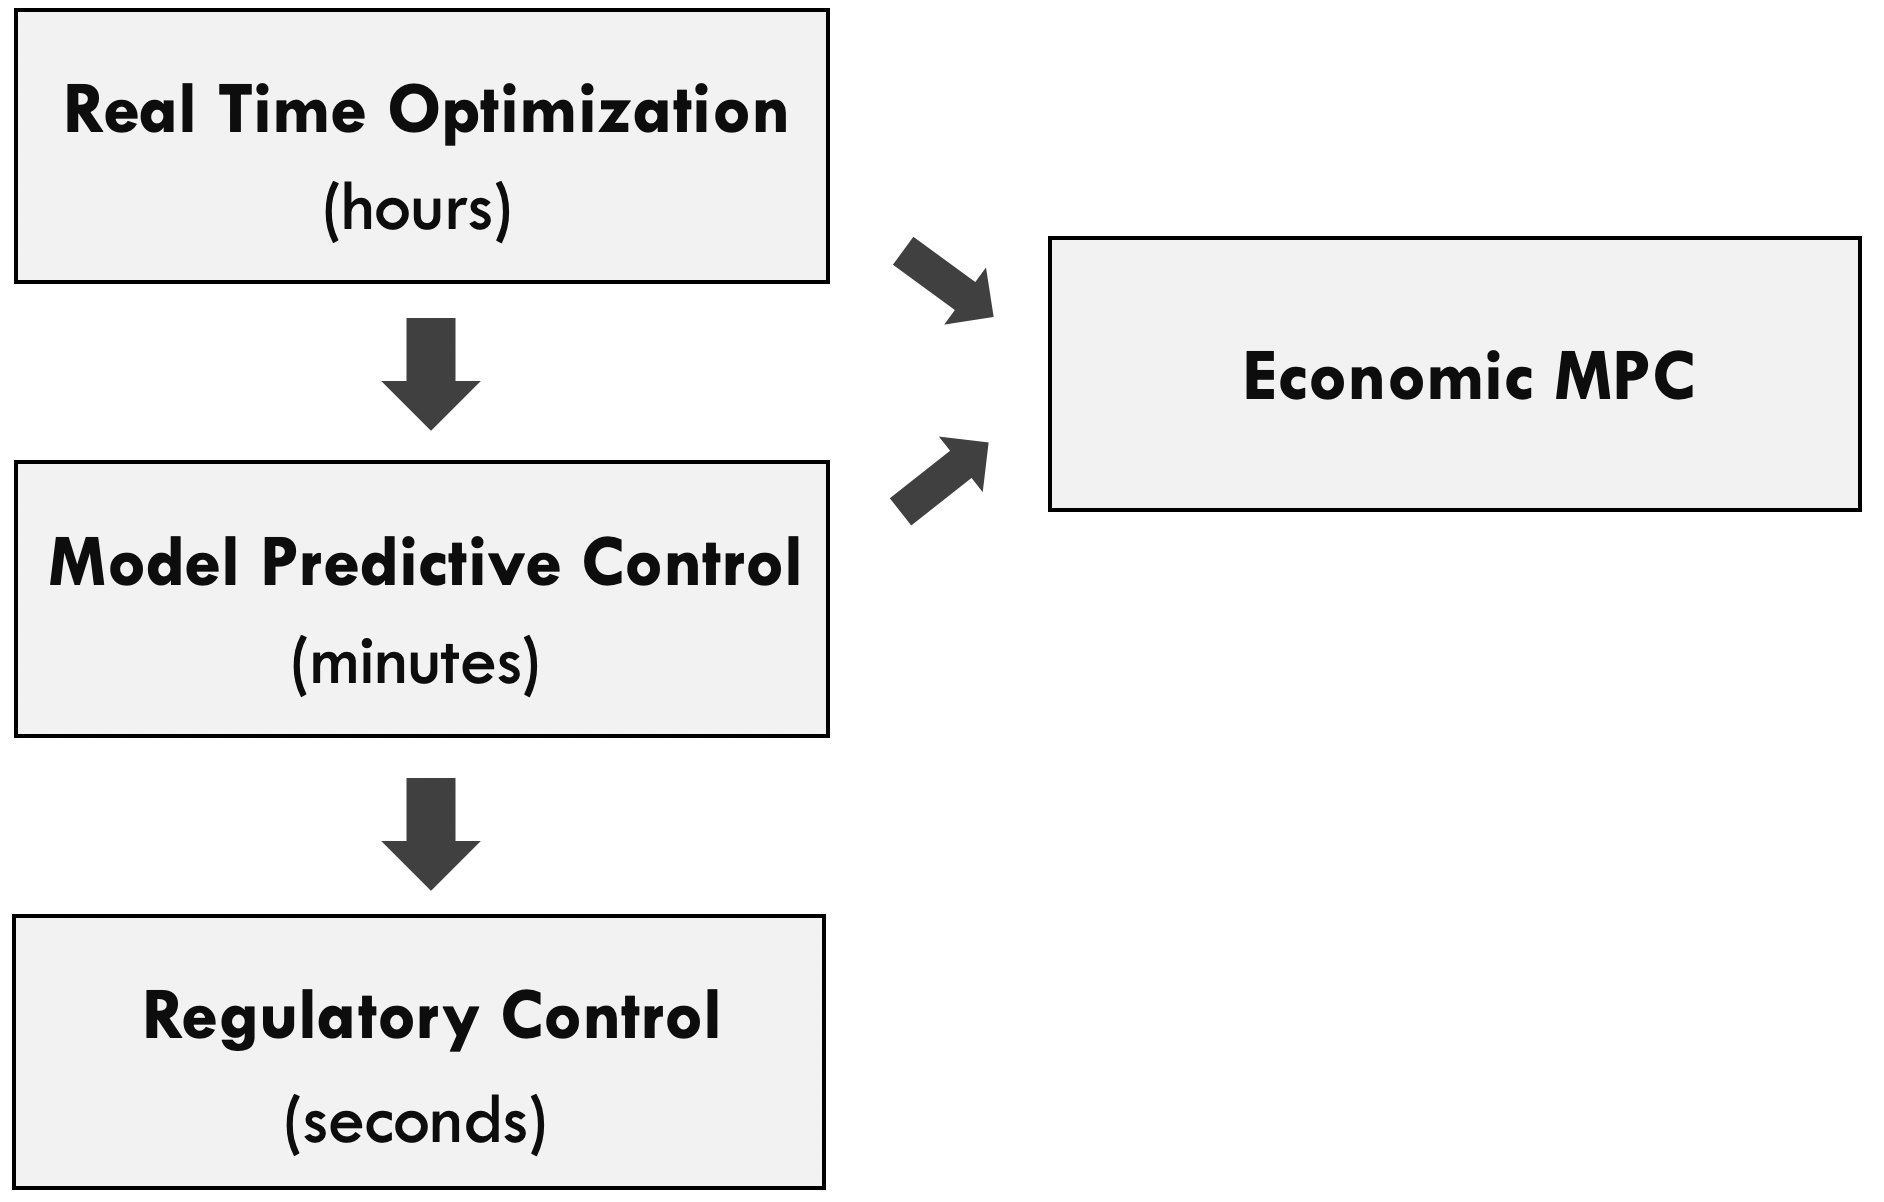
\includegraphics[width=0.5\textwidth]{images/ch1/rto_mpc_pid.jpeg}
    \caption{A typical industrial control architecture.}
    \label{fig:rto_mpc_pid2}
\end{figure}

In control literature, there typically exists very distinct algorithms for each layer presented in \ref{fig:rto_mpc_pid2}. For example, PID controllers are typically used for the regulatory layers whereas the supervisory layers typically employ predictive controls. Due to RL's general nature, it is highly flexible and can used in \textit{any} control layer. For example, a MPC RL agent's reward function is simply the negative of Equation \ref{eq:mpc}, with the actions being the control actions or recommended set points.  For a regulatory layer agent, the reward function remains the same, but the actions would involve direct actuation of the system's hardware.  Lastly, an EMPC based RL agent would have an economic objective as the reward function.

The \textit{biggest difference} between RL and other advanced control methods is the computation time. Typical MPCs have a computational complexity of $O(H(n^2 + m^2))$, where $H$, $n$, and $m$ are the control horizon and the dimensions of the states and actions, respectively \cite{mpc_comp_time}. By exploiting prior information, MPCs' computational complexity can further decrease to $O(H(n + m)^3)$ \cite{mpc_comp_time2, mpc_comp_time3, mpc_comp_time4}. Even then, the online computation time scales exponentially with states and actions, ultimately becoming infeasible for large systems and/or for systems with exceptionally long prediction/control horizons. Comparatively, RL's optimal policy is first pre-computed \textit{offline} through a training process.  Consequently, this makes online evaluation exceptionally quick.  In control theory, the concepts of RL are very similar to parametric programming from explicit MPCs \cite{explicit_MPC}.  Some may see the training requirement of RL as extremely unattractive; however, offline computation time is typically very flexible (i.e., offline computations can be done anywhere, anytime, on any machine) and does not matter so long as it is not unreasonably long (e.g., 1 month).

Another major difference between RL and MP-based methods is RL's \textit{model-free} nature.  In RL, a (representative) model is only required for initial training of the agent; online implementations are \textit{model-free}. Conversely, the system model is almost exclusively used in MPC. Inaccurate models are detrimental to control performance. In literature, a technique known as off-set free control overcomes this issue through online parameter re-adjustment \cite{offset_free_control}; however, the re-identification process does not work well for extremely noisy processes. Moreover, most plants experience process drift, where the processes slowly changes as a function of wear and tear.  RL can inherently adapt to such an issue through a gradual and smooth process.  MPCs, however, adapt using off-set free control or other model re-identification methods.  For such methods, the updates directly and completely change the model parameters at each sampling time.  For processes heavily corrupted by noise, the parameters at each update is most certainly incorrect. 

Lastly, tabular RL has very few hyper parameters. As long as reasonable learning rates are used, RL would work for most cases. Deep RL methods contain much more hyper parameters and are much more mathematically complex.  Without a doubt, the tuning of deep RL require many parameter sweeps; however, such details will be omitted here because deep RL may not be economically viable to implement in its current state. For MPC, adequate tuning of the $Q_{mpc}$ and $R_{mpc}$ matrices are often times paramount for optimal process control.  

A comparison between RL and MPC on various important categories is shown in Table \ref{tab:rl_mpc_dmc}. In addition to comparing RL and MPC in literature, RL was also compared to industrial-grade MPCs currently implemented onto many processes world wide. One popular MPC product in industry is AspenTech's signature DMCplus and DMC3 products \cite{aspen_dmcplus, aspen_dmc3}. When implementing such products in real life, the system model will never be perfect; therefore, only a near-optimal solution is possible. Additionally, the computation time for DMC is exceptionally high and is unviable for many non-linear systems. Comparatively, RL is not concerned with the structure of the system; however, identifying an optimal policy for noisy systems will be more difficult. Adaptation-wise, RL performs random actions to calibrate to the real system (an idea that \textit{sounds} dangerous for online processes). Interestingly, AspenTech's technology also performs such random actions for model calibration.  During commissioning, the controller is typically initialized in the \textit{smart step} mode, where the system  performs random step tests \textit{online} to calibrate the system model to the real process.  Afterwards, operators often switch the system to \textit{calibrate} mode.  In this mode, the system continues to perform step tests in a much more infrequent and lower in magnitude fashion. Such an adaptation paradigm is identical to RL, where exploration is initially plentiful, but is eventually annealed to near zero.  For an more mathematical comparison between RL and MPC, see \cite{rl_vs_mpc}.

The features of RL, academic MPC, and industrial MPC is shown in Table \ref{tab:rl_mpc_dmc}.

\begin{table}[H]
\caption{A comparison between RL, MPC in literature, and industrial MPC software.}
\centering
{\scriptsize
\begin{tabular}{c|c|c|c}
& \textbf{Reinforcement Learning}	& \textbf{Model Predictive Control} & \textbf{AspenTech DMC}\\
\hline
Performance             & Close to optimal			& Optimal with perfect model   &  Close to optimal \\
Online comp. cost		& Low			& High   &  High \\
Offline comp. cost		& Policy \& model identification			& Model identification   &  Model identification \\
Reliance on model         	& Only for training			& At all times   &  At all times \\
Online calibration		& Exploratory moves			&  Various methods   &  Exploratory moves \\
Sensitivity to tuning   & Low			& High   &  High \\
\label{tab:rl_mpc_dmc}
\end{tabular}}
\end{table}

%%%%%%%%%%%%%%%%%%%%%%%%%%%%%%%%%%%%%%%%%%%%%%%%%%%%%%%%%%%%%%%%%%%%%%%%%%%%%%%%%%%%%
% Fault-Tolerant Control System
%
%
% 
%  
% 
% 
% 
%%%%%%%%%%%%%%%%%%%%%%%%%%%%%%%%%%%%%%%%%%%%%%%%%%%%%%%%%%%%%%%%%%%%%%%%%%%%%%%%%%%

\section{Fault-Tolerant Control System}
While RL can only approach the performance of MPC in academic studies where MPC utilizes a perfect process model, are well designed, is given sufficient computational time, and uses state-of-the-art hardware for computations.  RL's generality, ease of use, and adaptive nature might create more value in industrial environments where engineers are time constrained and are tasked with assembling a "good enough" controller with limited hardware.

This section explores the generality and robustness of the RL algorithm, even when imperfectly designed and compares it to MPC for fault-tolerant control.  The algorithm from this study was then simulated on the Wood-Berry distillation tower from the University of Alberta under different actuator faults.

\subsection{Introduction}
All process equipment such as sensors and actuators may malfunction or breakdown during their operational lifetime. Hence, it is desirable to have a fault-tolerant control system (FTCS) to ensure sufficient performance during these impending failures. The application of FTCS in an industrial environment results in increased operation robustness and safety, while reducing operating costs due to fewer plant-wide shut downs \cite{ftc_book_ref1}. A typical FTCS contains two parts: i) Fault detection system (FDS) to identify the location and type of fault; ii) fault-tolerant controller (FTC) to operate the process safely during a fault.

Traditionally, a FTCS contain a variety of different controllers to handle different faults that may occur during online operations \cite{ftc_book_ref1}. Furthermore, PID controllers are generally used for FTC and are specially tuned to handle each fault specifically \cite{process_faults}. The traditional approaches work well in terms of safety, but the sheer number of controllers command a  high maintenance cost.  Moreover, the controllers must be re-tuned periodically for optimal performance due to unavoidable process drifts caused by wear and tear \cite{process_control_ref13}.

In this study, a reinforcement learning (RL) FTCS is proposed where different system faults are detected and mediated using a general controller. Additionally, the FTC can automatically adapt to process drift and new operating conditions. The FTCS' set-up is designed to be general enough to learn different faults using the same algorithm and will to reside on top of existing regulatory control systems.  Furthermore, the controller does not suffer greatly due to poor tuning or model plant mismatch; a trait plaguing traditional optimal controllers \cite{model_plant_mismatch}.  The proposed FTCS is implemented onto continuous multiple-input multiple-output (MIMO) systems with input constraints subject to actuator faults. RL FTCS were previously proposed for discrete systems, but not in the continuous case where transition dynamics are explicitly considered \cite{ftc_ex2_ref5, ftc_ex1_ref6}. To demonstrate this approach, the system outputs are assumed to be measurable and the system dynamics are assumed to be stable using a pre-designed controller under the fault-free case.  During normal operations, the FDS will learn the expected closed-loop behaviour of the system.  Behaviours heavily deviating from the expected states are used to identify faults. The FTC is activated during faults to operate the system using the non-faulty components.

\section{Preliminaries}
\subsection{System Description}
A class of continuous-time MIMO systems with constrained manipulated inputs is considered in this study and described in state space form by:
\begin{equation}
\dot{x}(t) = f(x(t), u(t) + \Tilde{u}(t))
\label{eq:system_states}
\end{equation}
\begin{equation}
y = h(x(t)) + \varepsilon(t)
\label{eq:system_output}
\end{equation}
where $x(t) \in {\mathbb{R}}^m$ denotes the state vector at time $t$, $u(t)$ denotes the inputs at time $t$, $y = (y_{1}, y_{2}, ..., y_{n}) \in {\mathbb{R}}^n$ denotes the output variables, and $\Tilde{u}(t)$ denotes the constrained manipulated input corresponding to actuator faults, which will be the focus of this study. Lastly, $\varepsilon \thicksim N(0, \sigma^2)$ denotes Gaussian noise in the measurements of the output variables.

\subsection{The Reinforcement Learning Problem}
Fig. \ref{fig:MDP_Setup} shows the RL paradigm. The overall RL problem was stated in detail in Chapter 1, and will only be briefly explained here. Starting from the top, the \textbf{environment} includes all factors the agent cannot arbitrarily change (the system in this study). The \textbf{agent} observes the \textbf{states} of the environment and performs control \textbf{actions} that transition the environment to new states while outputting a \textbf{reward} based on a desired performance metric. The reward guides the agent to the optimal policy. In control, reward is typically a function of the tracking error. The agent's decision making process is formalized in the Markov decision process.
\begin{figure}[H]
    \begin{center}
        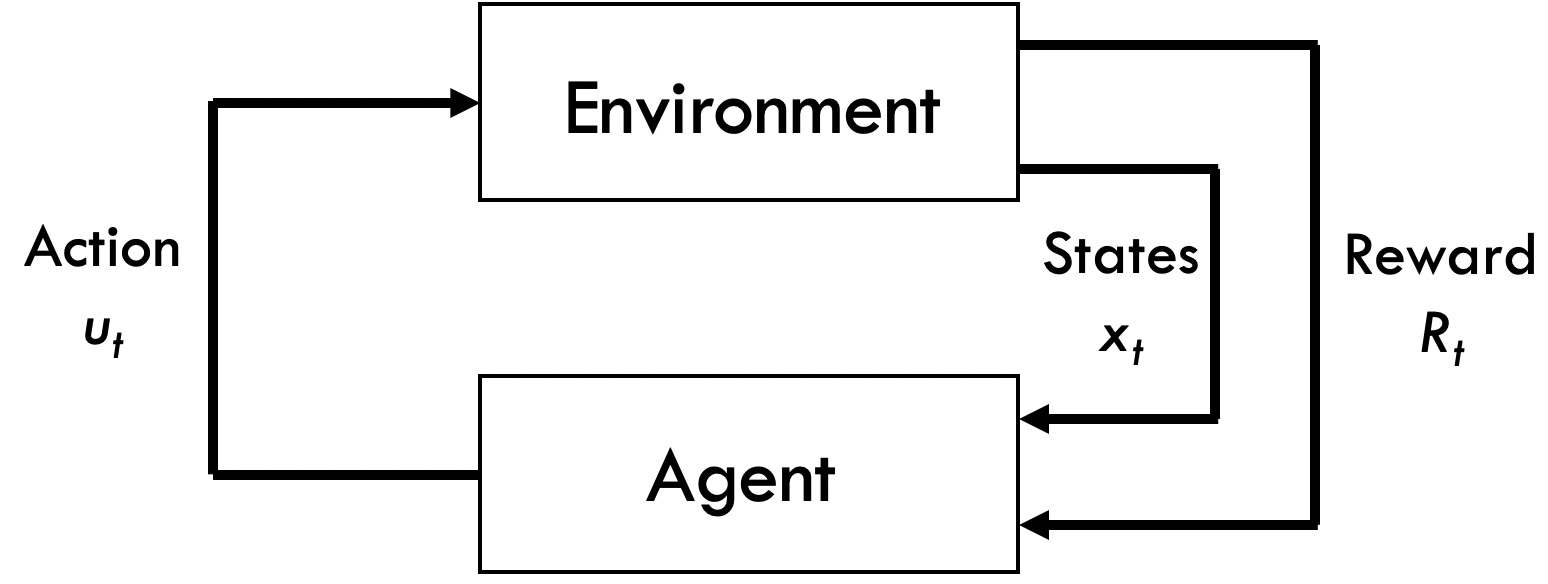
\includegraphics[width=11cm]{images/ftc/MDP_Setup.png}
        \caption{\label{fig:MDP_Setup} Paradigm of the reinforcement learning problem.}
    \end{center}
\end{figure}
\subsection{Markov Decision Process}
The Markov decision process (MDP) is a discrete representation of the stochastic optimal control problem and a classical formulation of sequential decision making \cite{sutton}.  MDPs provide formalism to agents when rationalizing about planning and acting in the face of uncertainty.  Many different definitions of MDPs exist and are equivalent up to small alternations of the problem.  One such definition is that a MDP, $\mathcal{M}$, is a tuple $(\mathcal{X}, \mathcal{U}$$, P(x', r|x, u), \gamma, R)$ comprised of \cite{ng_ref12}:
\begin{itemize}
    \item $x \in \mathcal{X}$: \textbf{State} space that describes the environment.
    \item $u \in \mathcal{U}$: \textbf{Action} space of the agent. ($     \mathcal{U}$ $ \geq 2 $)
    \item $R \in \mathbb{R}$: Expected \textbf{reward} from environment after agent performs $u$ in $x$. $|R| \; \leq \mathcal{R}$
    
    \item $P(x', r|x, u)$: \textbf{State transition probabilities} of the environment.  Given $x \in \mathcal{X}$, $u \in \mathcal{U}$, the probability of transitioning to $x'$ and receiving $r$.
    \item $\gamma$: \textbf{Discount factor} associated with future uncertainty.  ($0 \leq \gamma \leq 1)$
\end{itemize}
The agent starts in some initial states, $x_0$.  At each time $t$, the agent picks an action $u_t$ in accordance to the current policy $\pi$ and transitions to some $x_{t+1}$ while receiving $r_{t+1}$ drawn from the $P(x_{t+1}, r_{t+1} | x_t, u_t$).  By repeating the above procedure many times, the agent is able to traverse through some sequence $x_t, u_t, r_{t+1}, x_{t+1}, u_{t+1}, r_{t+2}, ...$ and accumulate:
\begin{eqnarray}
\begin{array}{rcl}
G_t = R_{t+1} + \gamma R_{t+2} + ... = \sum\limits^{\infty}_{k = 0} \gamma^k R_{t+k+1}
\end{array}
\label{eq:return}
\end{eqnarray}
where $G_t$ is the total discounted return along the sequence.  Here, the discount factor, $\gamma$, captures the uncertainty of future rewards and keeps $G_t$ bounded for non-terminating tasks. $R_t$ is the reward received at time $t$. The objective of the agent is to find the optimal control policy $\pi^*$, that maximizes $G_t$. Optimal solutions for MDPs work well for discrete tasks when transition times are constant and dynamics of the system are disregarded. However, such systems are rare in the process industry.  

Fig. \ref{fig:inv_overshoot_pid} shows different cases of poorly designed controllers in the process industry. Controllers resulting in oscillations, large overshoot, or severe inverse response lead to faster equipment deterioration and are detrimental to process safety \cite{process_control_ref13}. Additionally, transition time is often determined by the magnitude of change in the set-point in non-linear systems. Controllers typically require more time to track higher magnitude changes compared to ones of lower magnitude.  One could design a controller that evaluates seldomly to guarantee successful transitions, though such excessively conservative designs may lead to economic disadvantages.

\begin{figure}[H]
    \begin{center}
        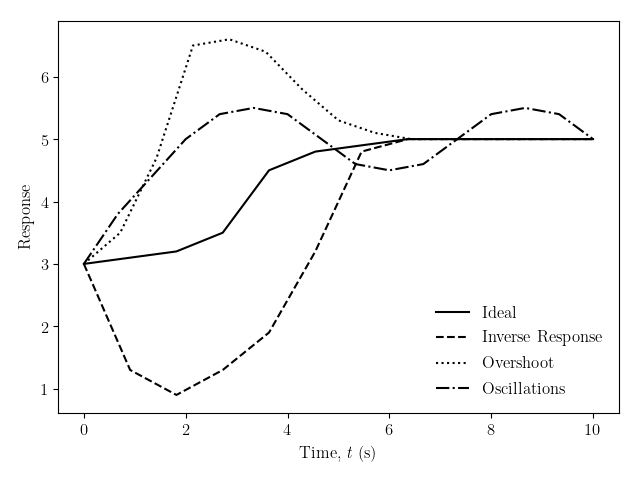
\includegraphics[width=9.5cm]{images/ftc/inv_overshoot_pid.png}
        \caption{\label{fig:inv_overshoot_pid} Symptoms of poorly designed controllers.}
    \end{center}
\end{figure}

\subsection{Semi Markov Decision Process}
System dynamics and transition times are vital to successful process control; therefore, continuous control problems with unknown transition times are formalized using the semi-Markov decision process (SMDP). In SMDPs, the dynamics of the transition period are captured using the reward \cite{continuous_rl_ref14}:
\begin{equation}
R(x_t, x_{t+1}, u_t) = \int\limits^\infty_0 \int\limits^t_0 e^{-\beta s} \rho(x, \pi (x))dsdF_{x, x_{t+1}}(t | \pi (x))
\label{eq:reward_rate}
\end{equation}
where $\rho(x, \pi (x))$ and $t$ are the average reward and transition time for the transition period from $x_t$ to $x_{t+1}$. Additionally, $\beta \in [0, \infty)$ is the discount factor for SMDPs.  High $\beta$ values result in short-sighted agents. $F_{x_t, x_{t+1}}(t | \pi_t)$ is the probability distribution of the time required for the system to transition from $x_t$ to $x_{t+1}$ given $\pi_t$.  The squared tracking error is calculated during intermediate transition periods, explicitly capturing transition dynamics during the search for $\pi^*$. Here, rewards for unknown transition time systems are corrected using:
\begin{eqnarray}
\begin{array}{rcl}
\gamma(x_t, x_{t+1}, u) = \int\limits^{\infty}_0 e^{-\beta t} dF_{x_t, x_{t+1}}(t | \pi_t)
\end{array}
\label{eq:discount_factor}
\end{eqnarray}

\section{Proposed Fault-Tolerant Control System}

Fig. \ref{fig:ftc_setup} shows the proposed FTCS for an arbitrary industrial process. The system contains three parts: i) Industrial process; ii) fault detection; iii) fault-tolerant control. The industrial process can be any arbitrary system (e.g., distillation tower, chemical reactor). A contextual bandit algorithm was used for the FDS. Subsequently, a tabular $Q$-learning approach was used for FTC. A bandit-based approach was selected for fault detection because the agent is not concerned with the long term reward (i.e., it is only concerned with the accuracy of its immediate classification) \cite{sutton}.  Contrarily, sequential decision making is critical for the success of an agent in control.  Thus, an RL-based agent was used for FTC \cite{bandits_ref9}. The tabular based approach was selected for its simplicity and ease of implementation into industrial distributed control systems (DCS), much like how explicit MPCs are implemented into processes that demand fast computations on cheap hardware with little storage \cite{explicit_MPC}. The flaws of the current algorithm are its lack of scalability and discrete nature.

For high dimensional industrial processes equipped with modern hardware, both scalability and discreteness can be eliminated by using deep Q-network (DQN) and deep deterministic policy gradient (DDPG) for the FDS and FTC, respectively.  DQN with $\gamma = 0$ is an ideal algorithm for the FDS due to its continuous state space and discrete action space. Likewise, DDPG is ideal for control due to its ability to handle large continuous states and action systems. For the remainder of this study, the contextual bandit agent used for fault detection and the RL agent used for FTC will be denoted as the \textit{prediction agent} and \textit{control agent}, respectively.

\begin{figure}[H]
    \begin{center}
        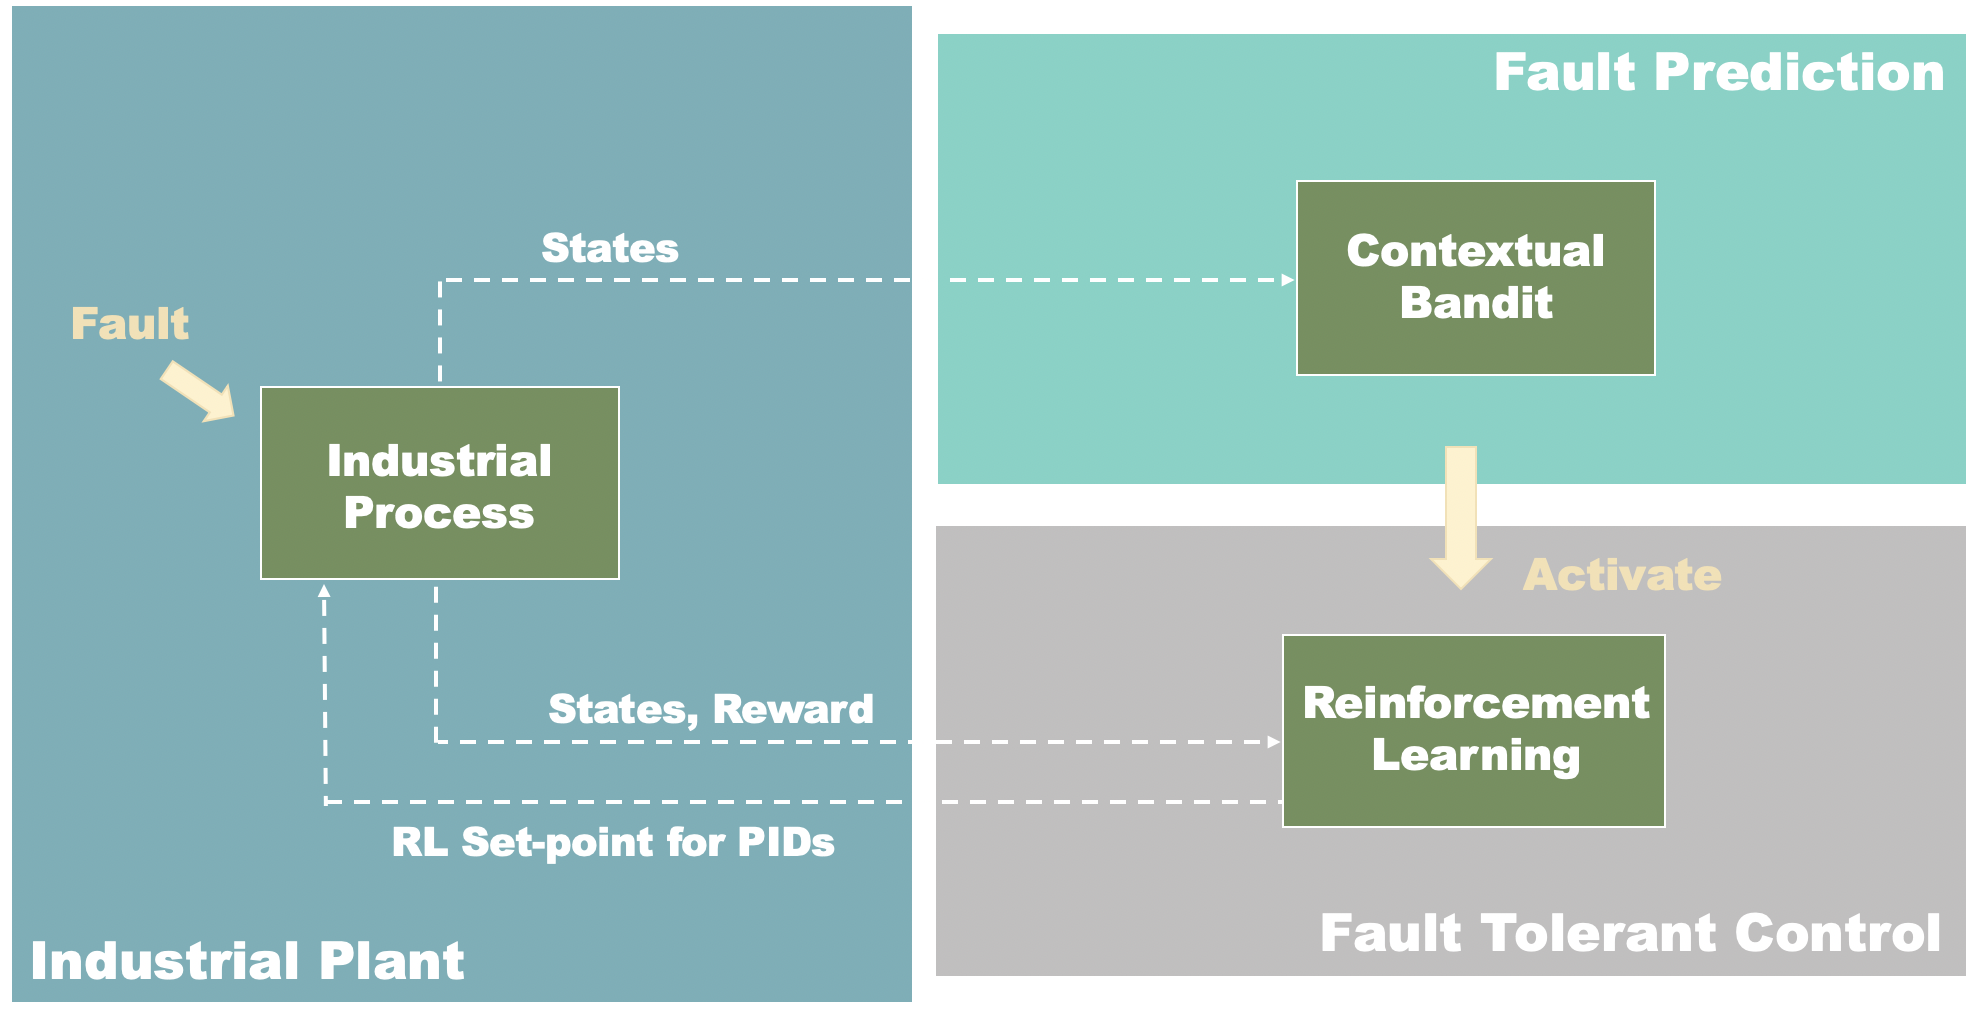
\includegraphics[width=11cm]{images/ftc/FTC_Setup.png}
        \caption{\label{fig:ftc_setup} Overall set-up of the fault-tolerant control system.}
    \end{center}
\end{figure}
In Fig. \ref{fig:ftc_setup}, the information flow is as follows.  Initially, the industrial process is operating fault-free while the prediction agent is actively monitoring real time measurements for faults.  When a fault is detected, the prediction agent will immediately activate the control agent to receive real time measurements from the process.  Given the current process off-set, the control agent gives recommendations to the operators regarding solutions to mediate the situation.  Recommendations can be new set-points for the regulatory controllers not at fault.
Fig. \ref{fig:ftc_pid_setup} shows the information flow of the control agent. 
\begin{figure}[H]
    \begin{center}
        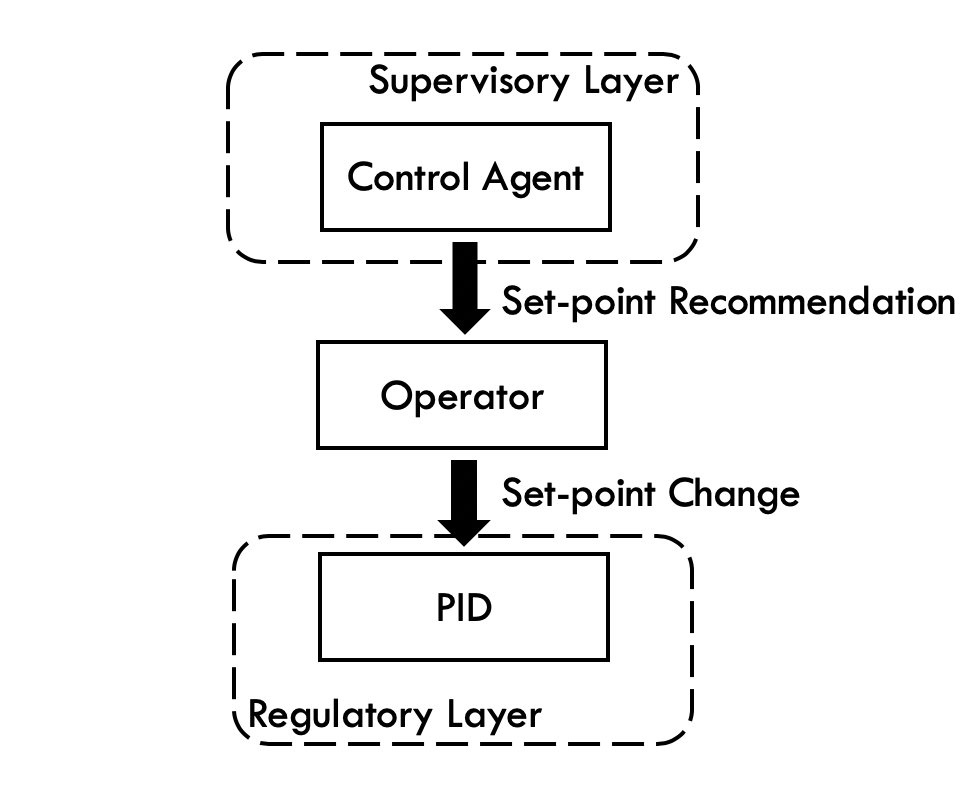
\includegraphics[width=9.5cm]{images/ftc/ftc_pid_setup.png}
        \caption{\label{fig:ftc_pid_setup} Information flow from the FTCS to the process.}
    \end{center}
\end{figure}
\subsection{Contextual Bandits Fault Detection}
The fault detection system is used to identify faults in the process.  FDS can be categorized as model-, knowledge- or prediction-based approaches \cite{ftcs_diagnosis_ref7}. Model-based approaches require an explicit model of the process.  A fault is deemed active if the prediction of the model is drastically different from the real time sensor measurement.  Knowledge-based approaches are based on subject matter expertise from process operators or equipment vendors and are usually rule-based (e.g., if $x > x_{max}$, then fault). Prediction-based approaches use historical data to identify a classification model for fault detection. The identified model would contain knowledge about normal operating boundaries regarding the process, and can be tuned by plant managers to be more conservative or aggressive. When the process conditions are outside the acceptable boundaries, a fault is deemed active. 

Prediction-based methods are quickly becoming the forefront approach due to more readily available data. This study uses a contextual bandit prediction-based FDS to identify process faults. A contextual bandit algorithm was selected due to its ability to adapt to non-stationary problems.  Furthermore, bandit-based algorithms are well suited for identification tasks because the agent is not concerned with long term reward \cite{sutton}. The objective of the agent is to identify if the current situation is faulty, given the current states $x_t$ of the process. 

\subsubsection{Prediction Agent Algorithm}

In contextual bandit problems, for each time $t$, the agent observes states $x_t$ and picks one action $u_t \in \mathcal{U}$.  After each action, a scalar reward feedback is sent to the agent as feedback to promote or discourage future similar state-action pairs.  For each action in state $x \in \mathcal{X}$, there is an expected reward called \textit{action value}, given by Equation (\ref{eq:value}).
\begin{equation}
    q^*(x, u) = {\mathbb{E}} [R_t | X_t = x, U_t = u]
    \label{eq:value}
\end{equation}
where $q^*(x, u)$ is the expected reward of taking $u$ in $x$. Here, $R_t$ is drawn from a distribution, $R_t \thicksim N(q_*(x, u), \sigma^2)$ \cite{sutton}. The real action-value is unknown, but can be estimated from Equation (\ref{eq:bandit_update}) \cite{bandits_ref9}.
\begin{equation}
    Q^{n+1}(x, u) \leftarrow Q^n(x, u) + \alpha_n (R_t - Q^n(x, u))
    \label{eq:bandit_update}
\end{equation}
where $Q(x, u)$ and $n$ are the estimate of $q^*(x, u)$ and the number of times $Q(x, u)$ was estimated prior to the current estimate.  $\alpha$ is the learning rate and is constant for adapting to non-stationary problems \cite{sutton}.  

Table \ref{tab:fds_reward} shows the reward space for the prediction agent. Furthermore, $\mathcal{U}$ and $\mathcal{X}$ are given by $Actions = [Fault, No \; Fault]$ and $[x^r_1, x^r_2, ..., x^r_v]$, respectively. Superscript $r$ and subscript $v$ denotes the relevant states and the number of relevant states, respectively.
\begin{table}[htb]
	\begin{center}
		\caption{\label{tab:fds_reward} Reward for the prediction agent.}
	\def\arraystretch{1.05}
	\begin{tabular}{p{5cm}p{3cm}p{3cm}p{0.01mm}}
	\hline
	 \centering Process Fault &  \centering Action &  \centering Reward & \\
	 \hline
	 \centering Yes & \centering Fault & \centering 1 & \\
	 \centering Yes & \centering No Fault & \centering -1 & \\
	 \centering No & \centering Fault & \centering -1  & \\
	 \centering No & \centering No Fault & \centering 0 & \\
	\hline
	\end{tabular}
	\end{center}
\end{table}
To train the prediction agent, first, the historical data must be labeled for faults. Next, the prediction agent will sample from the historical data and update its internal action values with accordance to Table \ref{tab:fds_reward}.
\begin{table}[htb]
    \begin{center}
	\def\arraystretch{1.1}
	\begin{tabular}{p{9cm}}
	\hline
	\textbf{Contextual Bandit:} \emph{Learn $f$: $\mathcal{X} \times \mathcal{U} \rightarrow \mathbb{R}$} \\ \hline
	    \textbf{\textit{Require:}} \\
	    States ${\mathcal{X}} = \{x_1, x_2, ..., x_v\}$ \\
	    Actions ${\mathcal{U}} = \{u_1, u_2\}$ \\
	    Reward Function $R: {\mathcal{X}} \times {\mathcal{U}} \rightarrow {\mathbb{R}}$ \\
	    Learning rate $\alpha \in [0, 1]$ \\
		\textbf{\textit{Procedure}} \textit{Contextual Bandit} $({\mathcal{X},\; \mathcal{U}},\; R, \; \alpha)$ \\
		\hspace{0.25cm} Initialize zero matrix $Q(x, u)_{{\mathcal{X}} \times {\mathcal{U}}}$ \\
		\hspace{0.25cm} \textbf{\textit{While}} Q not converged \textbf{do} \\
		\hspace{0.5cm} Sample state, $x_t$ \\
		\hspace{0.5cm} Pick $\argmax_{u_t} Q(x_t,u_t)^*$ \\
		\hspace{0.5cm} Perform action $u_t$, observe $R_{t+1}$ \\
		\hspace{0.5cm} $Q(x_t, u_t) \leftarrow Q(x_t, u_t) + \alpha(R_{t+1} - Q(x_t, u_t))$ \\ \hline
		*Note: Ties broken randomly to avoid bias.
	\end{tabular}
	\end{center}
\end{table}

Once $Q(x, u)$ reaches convergence, real time process measurements are sent to the prediction agent to detect potential faults. Action selection is given by:
\begin{equation}
    \centering
    u_t = \argmax_u Q_{\pi}(x, u), \; \forall \; x \in \mathcal{X}
    \label{eq: opt_policy}
\end{equation}

The prediction agent will activate the control agent when a fault is deemed active.

\subsection{Reinforcement Learning Fault-Tolerant Control}
Once activated, the control agent provides recommendations to stabilize the process.  Two strategies exist for the control agent: active FTC and passive FTC \cite{ftcs_passive_active_ref8}. Active FTC refers to re-configurable control, whereas passive FTC uses robust control principles. Active FTCs are generally more economically advantageous because passive FTCs are relatively more conservative. A tabular $Q$-learning active FTC is used for this study because of its adaptive nature and ability to acknowledge future rewards \cite{rl_control_ref10}. 

\subsubsection{Control Agent Algorithm}
Reinforcement learning is similar to contextual bandits with the alteration that the long term trajectory is also considered. The $Q$-learning algorithm for MDPs is:
\begin{equation}
    Q^{n+1}(x, u) \leftarrow Q^n(x, u) + \alpha_n(R_t + \gamma max_u' Q^n(x', u') - Q^n(x, u))
    \label{eq:q-learning}
\end{equation}
where $x'$ and $u'$ are the next state and the action that maximizes the return in $x'$. By combining Equation (\ref{eq:q-learning}) with Equations (\ref{eq:reward_rate}) and (\ref{eq:discount_factor}), SMDP $Q$-learning is given by:
\begin{equation}
    Q^{n+1}(x, u) \leftarrow Q^n(x, u) + \alpha_n \left[\frac{1 - e^{-\beta \tau}}{\beta}R_t + e^{-\beta \tau} max_{u'} Q^n(x', u') - Q^n(x, u) \right]
\label{eq:q-learning-smdp}
\end{equation}
where $R_t$ is given by Equation (\ref{eq:reward_rate}) and $\tau \leq \tau_{max}$ is the transition time from $x_{t}$ to $x_{t+1}$.  If $x_{t} \neq x_{t+1}$ at $\tau_{max}$, the agent evaluates regardless.  The reward is:
\begin{equation}
\rho= - \sum\limits^m_{k=1} (y_{k}(t) - y_{k}^{sp}(t))^2 = - \sum\limits^m_{k=1} e_k(t)^2
\label{eq:mse}
\end{equation}
where $y_{k}^{sp}(t)$ and $e_k(t)$ are the set-point and tracking error for $y_k$ at $t$.  The states and actions are discretized as: 
\begin{equation}
{\mathcal{X}} = [(e_{1}^{min}, ..., e_{m}^{min}), ..., (e_{1}^{max}, ..., e_{m}^{max})]_{p^2 \times 1}
\label{eq:states}
\end{equation}
\begin{equation}
{\mathcal{U}} = [(u_{1}^{min}, ..., u_{o}^{min}), ..., (u_{1}^{max}, ..., u_{o}^{max})]_{q^2 \times 1}
\label{eq:actions}
\end{equation}
where superscripts $min$ and $max$ denotes the min and max for each state error or action. $p, q \geq 2$ denotes the number of discretized values. 

During training, exploration of the environment is mandatory to avoid locally optimal policies. Traditional exploration methods, such as $\epsilon$-greedy, indiscriminately tries non-greedy actions (i.e., non reward maximizing actions given the current knowledge) with a fixed probability \cite{sutton}. However, exploring in frequently visited states makes little sense. Instead, it be better to select non-greedy actions based on their potential of being optimal. One such way to do this is to use UCB action selection \cite{sutton}:
\begin{equation}
    U_t = \argmax_u \left[Q_t(x, u) + c \sqrt{\frac{ln \; t}{N_t(x, u)}} \right]
\label{eq:ucb}
\end{equation}
where $ln \; t$ and $c$ are the natural logarithm of $t$ and the exploratory factor, respectively. Large $c$ values result in more exploration. $N_t(x, u)$ is the number of times $u$ is picked in $x$ prior to $t$.  The square root term is the measure of uncertainty in the current $Q$ values.  Uncertainty is reduced each time $u$ is selected by increasing $N_t(x, u)$.

The control agent is trained using a high-fidelity simulator for the system.
\begin{table}[H]
    \begin{center}
	\def\arraystretch{1.05}
	\begin{tabular}{p{12cm}}
	\hline
	\textbf{UCB Q-Learning:} \emph{Learn $f$: $\mathcal{X} \times \mathcal{U} \rightarrow Q$} \\ \hline
	
		\textbf{\textit{Require:}} \\
	    States ${\mathcal{X}} = \{x_1, x_2, ..., x_m\}$ \\
	    Actions ${\mathcal{U}} = \{u_1, u_2, ..., u_o\}$ \\
	    Reward function $R: {\mathcal{X}} \times {\mathcal{U}} \rightarrow {\mathbb{R}}$ \\
	    Learning rate $\alpha \in [0, 1]$ \\
	    SMDP discount factor $\beta \in [0, \infty)$ \\
	    Degree of exploratory $c \in [0, \infty)$ \\
		\textbf{\textit{Procedure}} \textit{UCB Q-learning} $({\mathcal{X},\; \mathcal{U}},\; R, \; \alpha, \; \beta, \; c)$ \\
		\hspace{0.25cm} Initialize zero matrices $Q(x, u)_{{\mathcal{X}} \times
		{\mathcal{U}}}$, $N(x, u)_{{\mathcal{X}} \times {\mathcal{U}}}$ \\
		\hspace{0.25cm} Initialize time, $t_0$ \\
		\hspace{0.25cm} Observe initial state, $x_0$ \\
		\hspace{0.25cm} \textbf{\textit{While}} Q is not converged \textbf{do} \\
		\hspace{0.5cm} Pick $\argmax_{u_t} Q(x_t,u_t) + c \sqrt{\frac{ln \; t}{N(x, u)}} ^*$ \\
		\hspace{0.5cm} Perform $u_t$, expect $x_{t+1}$ \\
		\hspace{0.5cm} When $x \approx x_{t+1}$, observe $R(x_t, x_{t+1}, u_t), \tau$ \\
        \hspace{0.5cm} $Q(x_t, u_t) \leftarrow Q(x_t, u_t) + \alpha \left[\frac{1 - e^{-\beta \tau}}{\beta}R \; + ... \right.$ \\
        \hspace{1.7cm} $\left. e^{-\beta \tau} max_{u_{t+1}} Q(x_{t+1}, u_{t+1}) - Q(x_t, u_t) \right]$ \\
		\hspace{0.5cm} $N(x, u) \leftarrow N(x, u) + 1$; \; $x_t \leftarrow x_{t+1}$; \; $t \leftarrow t + 1$ \\ \hline
		*Note: Ties broken randomly to avoid bias.
	\end{tabular}
	\end{center}
\end{table}
After convergence of $Q(x, u)$, $c$ is set to zero to stop exploration. Actions are picked using:
\begin{equation}
u_{i, t} = u_{i, t - 1} + \Delta u_{i, t}, \hspace*{0.3cm} u_{i}^{min} \leq u_{i, t} \leq u_{i}^{max}
\label{eq:velocity_controller}
\end{equation}
where $\Delta u_t$ is from Equation (\ref{eq: opt_policy}).

\subsection{Stability and Convergence}
The stability of RL is guaranteed assuming a Lipschitz continuous model and confining exploration to within the region of attraction, given a bounded input \cite{stability_rl_ref21}. For convergence, given learning rates $0 \leq \alpha_n < 1$, bounded rewards $|r_n| \leq \mathcal{R}$ and:
\begin{equation}
    \sum\limits^{\infty}_{i = 1}\alpha_i(x, u) = \infty, \; \;  \sum\limits^{\infty}_{i = 1}\alpha_i^2(x, u) < \infty, \forall x, u,
\end{equation}
the tabular $Q$-learning values, $Q_n(x, u) \rightarrow Q^*(x, u)$ as $n \rightarrow \infty, \forall x, u$ with probability 1---the optimal result given such stochastic conditions \cite{convergence_rl_ref20}.

Fig. \ref{fig:08RL_implementation} shows the steps to implementing the control agent into industrial control systems for mediating faults in \textbf{stable} processes where the above conditions are satisfied. The implementation consists of three phases: i) preliminary training, ii) calibration; iii) online monitoring. 

\begin{itemize}
    \item \textbf{Preliminary training:}  A seed model of the process is first identified to allow for preliminary control agent training. Simulations using the seed model will establish a baseline performance for control agent. In this step, the control agent will learn to operate the process under a desired performance metric without using the commonly faulty equipment to gain fault tolerance.
    \item \textbf{Calibration:} The simulation-trained control agent will be implemented online where it will operate and adapt to the real process, overcoming any model plant mismatch. The control agent will perform minuscule exploratory moves while online to ensure optimality.  Exploratory moves can be tuned by $u_{e, min} \leq u \leq u_{e, max}$, where $u_{e, min}$ and $u_{e, max}$ are the lower and upper bounds of the exploratory actions.
    \item \textbf{Online monitoring:} After sufficient performance is achieved, exploration will be terminated, and the control agent is ready to mediate process faults.
\end{itemize}

\begin{figure}[H]
    \centering
    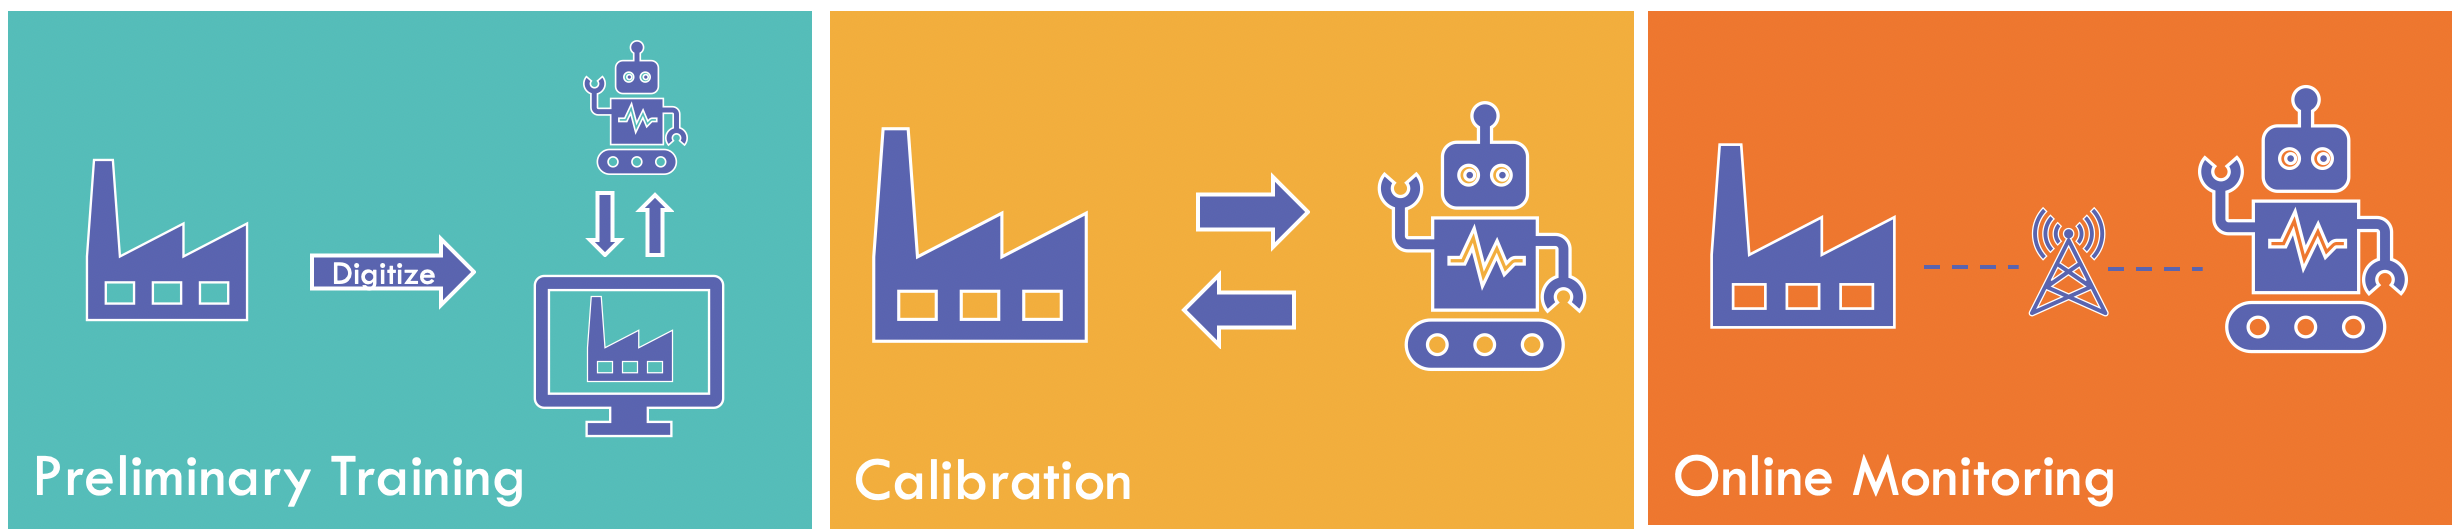
\includegraphics[width=12cm]{images/ftc/rl_implementation.png}
    \caption{Steps on implementing the control agent.}
    \label{fig:08RL_implementation}
\end{figure}

The plant managers may choose to leave the control agent in calibrate mode during a fault so it can continue to identify more optimal control strategies.  Such a strategy sounds risky in academia; however, it is indeed how state-of-the-art MPCs are implemented in industry.

\subsection{Computational Complexity}
The computation complexity was decomposed into training complexity and online evaluation complexity.  The training complexity refers to the computational time to find the optimal policy.  Likewise, the online evaluation complexity is the online evaluation time required to find the optimal input.  Assuming \textit{tabula rasa}, the computational complexity to reach the goal state for the first time during training is $O(p^3)$ \cite{complexity_rl_ref19}. Online evaluation complexity is approximately $O(mlog(p))$ and $O(mlog(p) + qlog(q))$ for the prediction and control bandit, respectively. Here, the $O(mlog(p))$ is associated with finding the index of the states using binary search.  Similarily, $O(qlog(q))$ refers to sorting the value functions using heap sort to find the maximum value. For traditional optimal control solvers, the computational complexity is $O(N^3(p + q)^3)$, where $N$ is the control horizon \cite{mpc_comp_time}. Comparatively, RL evaluates much faster online compared to traditional optimal control methods, but must first be trained. For tasks where long training times are feasible and demand fast online evaluation times, reinforcement learning may be the superior choice.  Typically in the process control industry, training models offline is not a significant downfall; however, online evaluation time is incredibly scarce especially in highly complex plants due to hardware limitations.  Therefore in terms of computation, RL may be the desired method.

\section{Case Study}
The proposed FTCS was simulated on a distillation tower to illustrate the pros and cons compared to traditional methods. Distillation towers are integral units in industrial processes that require the separation of
mixtures of different components into products based on their relative volatility. Heavy oil
upgrading facilities utilize distillation towers to separate feed mixtures into various products based on their specific gravity.  For many chemical plants, the distillation tower can account up to 50\% of the total operating cost, making optimization of the distillation tower a low hanging fruit for cost savings.  

Flooding is a common and costly problem in industrial distillation towers.  Flooding occurs when liquids are entrained in the vapour due to abnormally high vapour flow rates.  Moreover, the excess pressure also causes liquid holdup in the higher plates of the distillation tower. Ultimately, this leads to significant reduction in separation efficiency causing a loss in production, wasted energy, and off-spec products. Flooding commonly occurs when the distillation tower heats up uncontrollable; typically due to actuator faults.  In this case study, the proposed FTCS will be applied to the Woodberry distillation tower under different actuator faults. The FTCS will reside in the supervisory control layer, outputting recommended set-points for the regulatory controllers.

\subsection{Process Description}
Distillation is the process of separating a liquid or vapour mixture of two or more components into desirable purities through the addition or removal of heat. The fundamental theory of distillation is that low boiling point components are richer in the vapour of a boiling mixture, while the liquids would contain more of the less volatile components \cite{distillation_intro}.  Liquids exit the bottom of the distillation tower and is sent to a reboiler, where heat is added to vaporize any straggling high volatility product to ensure maximum separation. Similarly, vapour from the top of the tower is sent to a condenser, where heat is removed and additional low volatility components may be recovered. The condensed vapour is collected in the reflux drum, and will be recycled back into the distillation tower. Typically, distillation columns are large vertical drums with evenly spaced trays to enhance separation of the vapour and liquid components \cite{mpc_for_distillation_tower}.  The tower is separated into two sections.  The rectifying section is located between the feed tray and the top of the column and aims to concentrate light components in the vapour phase.  Moreover, the stripping section is located between the feed tray and the column bottom and is used to concentrate the heavier components in the liquid phase \cite{henry_distillation}.

The Wood-Berry distillation tower, shown in Fig. \ref{fig:woodberry}, contains one feed stream and two outlet streams. The feed stream containing methanol and water is characterized by the inlet mass composition $Z_f$. Methanol has a boiling point of 64.7 \textdegree C whereas pure liquid water has a boiling point of 100 \textdegree C \cite{sonntag_thermo}. Thus, making methanol the distillate and water is the bottoms product. The control inputs are the reflux and steam flow rates, $R \; (lb/min)$ and $S \; (lb/min)$. Furthermore, the outputs are characterized by the distillate and bottoms methanol mass fraction, $X_D$ and $X_B$, respectively. Objectively, the distillation column aims to achieve 100\% $X_D$, while maintaining $X_B$ at 0\%. Additional detailed information about the operation and inner workings of distillation towers can be found in \cite{henry_distillation}.  
\begin{figure}[H]
    \begin{center}
        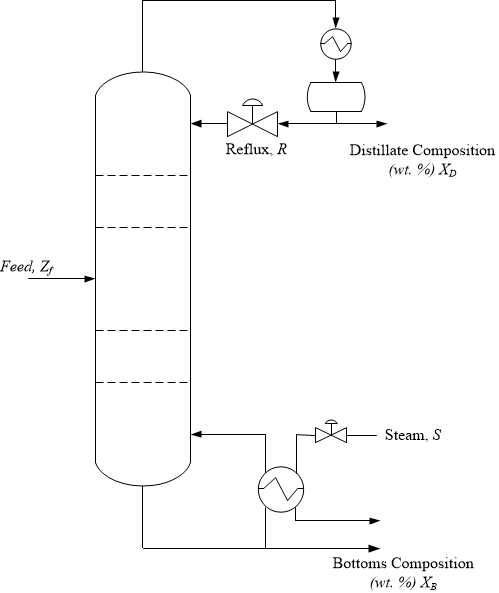
\includegraphics[width=9cm]{images/ftc/woodberry.png}
        \caption{\label{fig:woodberry} Wood-Berry distillation tower schematic.}
    \end{center}
\end{figure}

The transfer function realization of the Wood-Berry distillation tower is given by Equation (\ref{eq:woodberry_tf}) \cite{woodberry_ref15}.
\begin{equation}
    \begin{bmatrix}
        Y_1(s) \\
        Y_2(s) 
    \end{bmatrix}
    =
    \begin{bmatrix}
        G_{11}  & G_{12} \\
        G_{21}  & G_{22}
    \end{bmatrix}
    \begin{bmatrix}
        u_1(s) \\
        u_2(s)
    \end{bmatrix}
\label{eq:woodberry_tf}
\end{equation}
where $u_1$ and $u_2$ are $R$ and $S$, respectively. $G_{ij}$ are: \\
\begin{equation}
    \begin{matrix}
        G_{11} = \frac{12.8e^{-s}}{16.7s + 1}     &     G_{12} = \frac{-18.9e^{-3s}}{21s + 1} \\
        G_{21} = \frac{6.6e^{-7s}}{10.9s + 1}     &     G_{22} = \frac{-19.4e^{-3s}}{14.4s + 1} \\
    \end{matrix}
    \label{eq:transfer_functions}
\end{equation}
Equation (\ref{eq:transfer_functions}) was converted into state space form using the $ss$ function in MATLAB and given by:

\begin{equation}
    \begin{bmatrix}
        \dot{x_1} \\
        \dot{x_2} \\
        \dot{x_3} \\
        \dot{x_4} 
    \end{bmatrix}
    =
    \begin{bmatrix}
        -0.06     &     0     &     0     &     0 \\
        0           &  -0.09  &     0     &     0 \\
        0           &     0     &   -0.05 &     0 \\
        0           &     0     &     0     &  -0.07
    \end{bmatrix}
    \begin{bmatrix}
        x_1 \\
        x_2 \\
        x_3 \\
        x_4 
    \end{bmatrix}
    + \\ I
    \begin{bmatrix}
        u_1(t - 1) \\
        u_1(t - 7) \\
        u_2(t - 3) \\
        u_2(t - 3)
    \end{bmatrix}
    + I
    \begin{bmatrix}
        \Tilde{u}_1(t - 1) \\
        \Tilde{u}_1(t - 7) \\
        \Tilde{u}_2(t - 3) \\
        \Tilde{u}_2(t - 3)
    \end{bmatrix}
    \label{eq: x_ss_eq1}
\end{equation}
\begin{equation}
    \begin{bmatrix}
    X_D \\
    X_B
    \end{bmatrix}
    =
    \begin{bmatrix}
    0.8 & 0 & -0.9 & 0 \\
    0 & 0.6 & 0 & -1.4
    \end{bmatrix}
    \begin{bmatrix}
    x_1 \\
    x_2 \\
    x_3 \\
    x_4 \\
    \end{bmatrix}
    +
    \begin{bmatrix}
    \varepsilon_1 \\
    \varepsilon_2 \\
    \varepsilon_3 \\
    \varepsilon_4 \\
    \end{bmatrix}
    \label{eq: x_ss_eq2}
\end{equation}
where $I$ is the identity matrix and $\Tilde{u}(t)$ denotes actuator faults. Initially, the system was at steady state where $X_D, X_B = 100, 0$ and initial states $x_0 = [251, 0, 103, 0]$. Measurement noises, $\varepsilon_i$, were sampled from $\varepsilon_i \thicksim N(0, 2)$. Applying the Popov-Belevitch-Hautus test to the system, $rank([B, AB, A^2B, A^3B]) = 4$, satisfying the controllability criterion \cite{process_control_ref13}.  Furthermore, it can be seen that $X_D$ and $X_B$ are controllable using either $u_1$ or $u_2$. Thus, even if one controller is faulty, the non-faulty controller can still guide one system output to the desired set-point.  Finally, the system matrix contains only negative eigenvalues; therefore, the system is globally asymptotically stable with the region of attraction spanning the entire state space.  Given a constrained input, the control agent in this study is guaranteed to be stable under any policy.

\subsection{Tuning of Regulatory Control}
Proportional-Integral (PI) controllers were used for regulatory control because its performance exceeds Proportional-Integral-Derivative (PID) controllers in the Wood-Berry distillation tower due to the slow dynamics of the system \cite{process_faults}. The discrete PI controller formulation is \cite{process_control_ref13}:
\begin{equation}
u_t = u_{t - 1} + K_p(e_t + e_{t - 1}) + K_i e_t
    \label{eq:PI}
\end{equation}
where $K_p$ and $K_i$ are the proportional and integral parameters that must be tuned. A multi-loop tuning strategy using equivalent transfer functions and simplified internal model control was used to tune the PI controllers \cite{decoupler_design}. The controller parameters are given in Table \ref{tab:PI_parameters}:
\begin{table}[htb]
	\begin{center}
		\caption{\label{tab:PI_parameters}Parameters for the PI controllers}
	\def\arraystretch{1.00}
	\begin{tabular}{p{1.5cm}p{1.5cm}p{1.5cm}p{0.01cm}}
	\hline
	 & \centering $u_1$ & \centering $u_2$ & \\
	 \hline
	 \centering $K_p$ & \centering 1.31 & \centering -0.28 & \\
	 \centering $K_i$ & \centering 0.21 & \centering -0.06 & \\
	\hline
	\end{tabular}
	\end{center}
\end{table}
\subsection{Fault-Tolerant Control System}
Integral wind-up is a common problem in PI controllers during actuator saturation or faults.  Amid these events, the integral term accumulates a larger error, often resulting in excessive overshooting and irresponsiveness to errors in the opposite direction \cite{process_control_ref13}. In this study, the prediction agent learned faults through large integral wind-ups.  The states of the prediction agent is ${\mathcal{X}} = [\Delta y_1, \Delta y_2, \Delta u_1, \Delta u_2]$. The prediction agent will learn typical $\Delta y_{1, 2}$ pairings with $\Delta u_{1, 2}$; if large $\Delta u_{1, 2}$ are observed without an equal change in $\Delta y_{1, 2}$, a fault is deemed active.

Fig. \ref{fig:FDS} shows the normal and faulty controller input-output pairing for $u_1$ and $X_D$. Points within the dashed circles are expected states from the closed-loop system. Any points residing outside are faulty. A similar relation exists with all other input-output pairings. The prediction agent will deemed a fault active when ten consecutive points fall outside the boundaries. This condition was imposed to prevent false alarms caused by noisy process data.
\begin{figure}[H]
    \begin{center}
        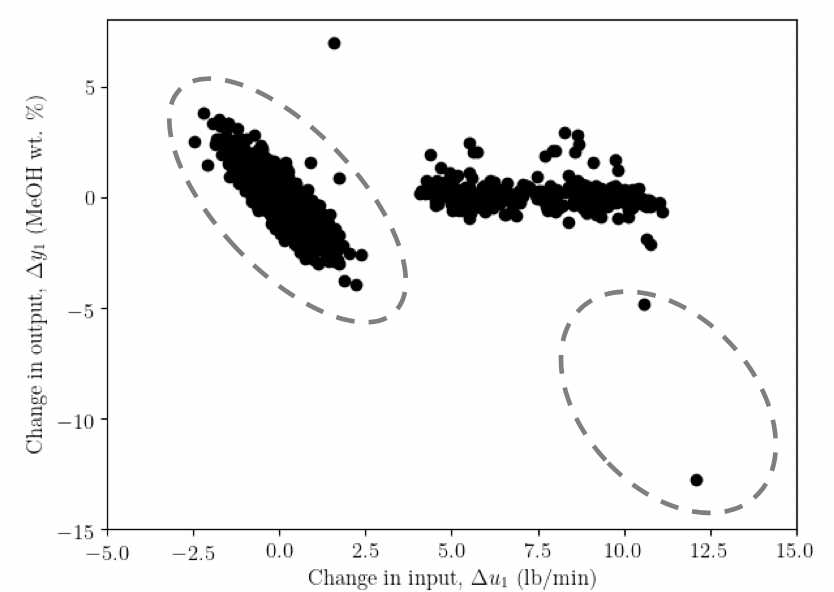
\includegraphics[width=10cm]{images/ftc/Boundaries.png}
        \caption{\label{fig:FDS} Relationship between $X_D$ and $u_1$.}
    \end{center}
\end{figure}

After a fault is identified, the control agent is activated to guide the system back to the fault free case, if possible. In this study, the control agent's state and actions are:
\begin{equation}
{\mathcal{X}} = [(-15, 15), (-15, -14), ..., (15, 15)]_{31^2 \times 1}
\label{eq:states_case_study}
\end{equation}
\begin{equation}
{\mathcal{U}} = [(-10, -10), (-10, -9), ..., (10, 10)]_{21^2 \times 1}
\label{eq:actions_case_study}
\end{equation}
Initial learning rate $a_0$, discount factor $\beta$, and exploratory factor $c$ were 0.5, 0.1 and 1.2, respectively. $\alpha$ is decayed as the agent gains experience, given by:
\begin{eqnarray}
\left\{
\begin{matrix}
    \alpha_t = a_0, & N(x, u) < 25 \\
    \alpha _t = \frac{\alpha_0}{1 + N(x, u)}, & N(x, u) \geq 25 \\
\end{matrix} \right.
\label{eq:learning_rate}
\end{eqnarray}
where $\alpha_t \in [0.001, 0.5)$. The reward, $|R| \; \leq 900$, is bounded and given by Eq. \ref{eq:mse}.  Learning rate decay and bounded reward are necessary for RL convergence \cite{convergence_rl_ref20}.
\subsection{Case Studies}
Table \ref{tab:case_studies} shows the four case studies that were explored.  The prediction and control agents were trained in simulation for 320,000 training steps for each case. A random actuator fault was introduced at the $150^{th}$ minute. $\tau_{max}$ was set to 30 minutes. Each episode was limited to a maximum of 2000 minutes before the system was reset. The PI controllers were evaluated every 4 minutes.
\begin{table}[htb]
	\begin{center}
		\caption{\label{tab:case_studies} Case studies for the FTCS}
	\def\arraystretch{1.3}
	\begin{tabular}{p{1.8cm}p{4cm}p{5cm}}
	\hline
	 & Reward & Description \\
	 \hline
	 Case 1 & - $e_{X_D}^2$ & Set-point Change \\
	 Case 2 & - $e_{X_B}^2$ & Set-point Change \\
	 Case 3 & - $0.8e_{X_D}^2$ - $0.2e_{X_B}^2$ & Optimal Operation \\
	 Case 4 & - $e_{X_D}^2  \rightarrow - e_{X_B}^2$ & Adaptation \\
	\hline
	\end{tabular}
	\end{center}
\end{table}

The case study simulation results are shown in Figs. \ref{fig:case_study1}, \ref{fig:case_study2}, \ref{fig:case_study3}, and \ref{fig:case_study4}. In case 1, the operator changed the set-point from $100\%$ to $90\%$ for $X_D$ at $t = 350$; however, the reflux valve became stuck. The FDS detected ten consecutive anomalous $( \Delta y_{1, 2}, \Delta u_{1, 2})$ pairs and activated the FTC which guided the system to the desired set-point successfully within 60 minutes. The FTC can also reject disturbances as shown at $t = 1400$. Without the FTCS, the system would have been stuck at $X_D = 76$.  Additionally, the system is robust to large process uncertainty (as shown in the noisy measurements). Likewise, Fig. \ref{fig:case_study2} shows a similar scenario for $X_B$ where the steam valve became stuck.  By training the FTCS for faults in $X_B$, the system can be easily re-stabilized using the \textit{same} algorithm and hyper parameters.

\begin{figure}[H]
    \begin{center}
    \begin{subfigure}[b]{0.49\textwidth}
        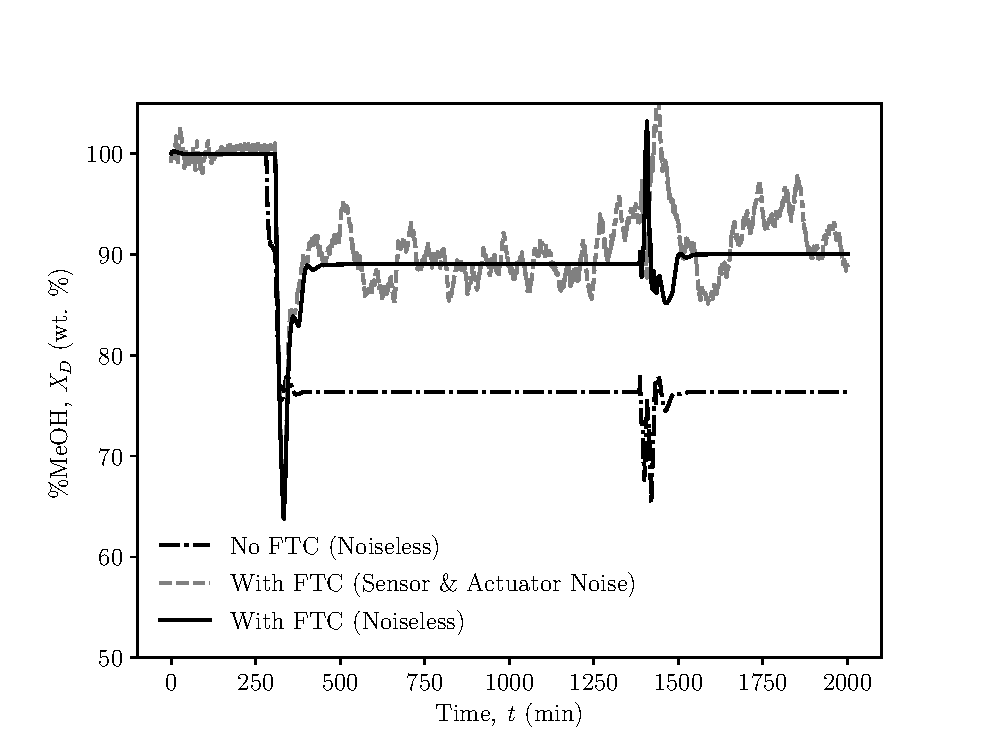
\includegraphics[width=\textwidth]{images/ftc/Case1_Plot.eps}
        \caption{\label{fig:case_study1} Fault in the reflux valve (Case 1).}
    \end{subfigure}
    \hfill
    \begin{subfigure}[b]{0.49\textwidth}
        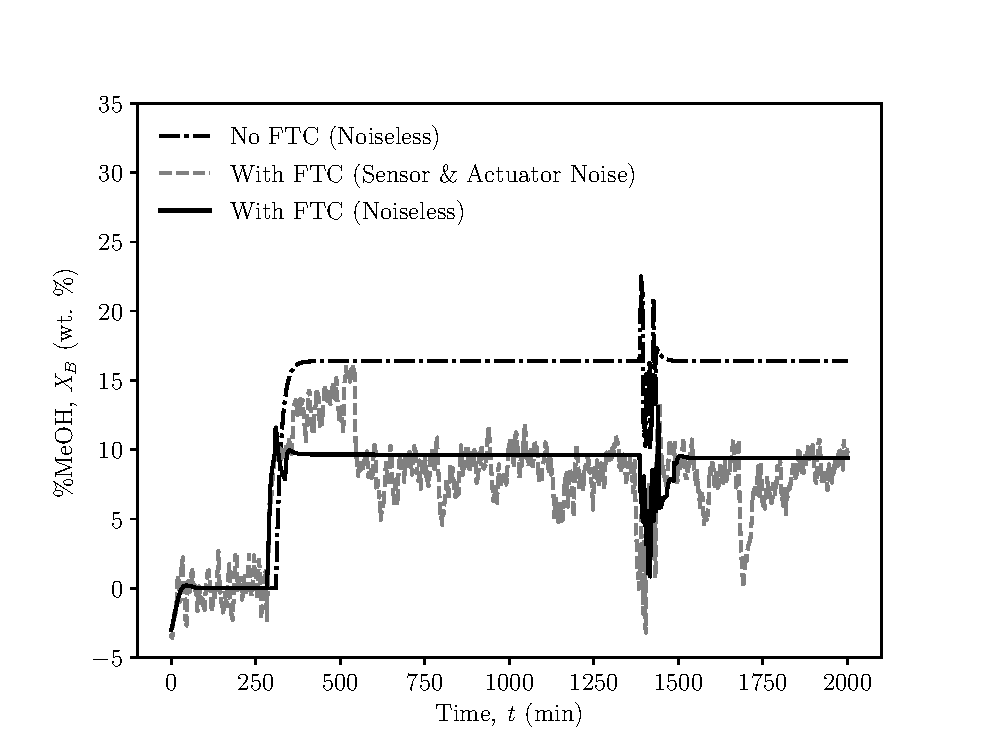
\includegraphics[width=\textwidth]{images/ftc/Case2_Plot.eps}
        \caption{\label{fig:case_study2} Fault in steam valve (Case 2).}
    \end{subfigure}
    \end{center}
\end{figure}

In case 3, both $X_D$ and $X_B$ are considered at different degrees, with $X_D$ being valued at four times greater than $X_B$.  During operations, an actuator fault occurred in the reflux valve, significantly impacting both $X_D$ and $X_B$.  With the remaining actuator, the system cannot be guided to the optimal set-points for both $X_D$ and $X_B$. Here, the agent found an operating condition to minimize the overall loss.

\begin{figure}[H]
    \begin{center}
        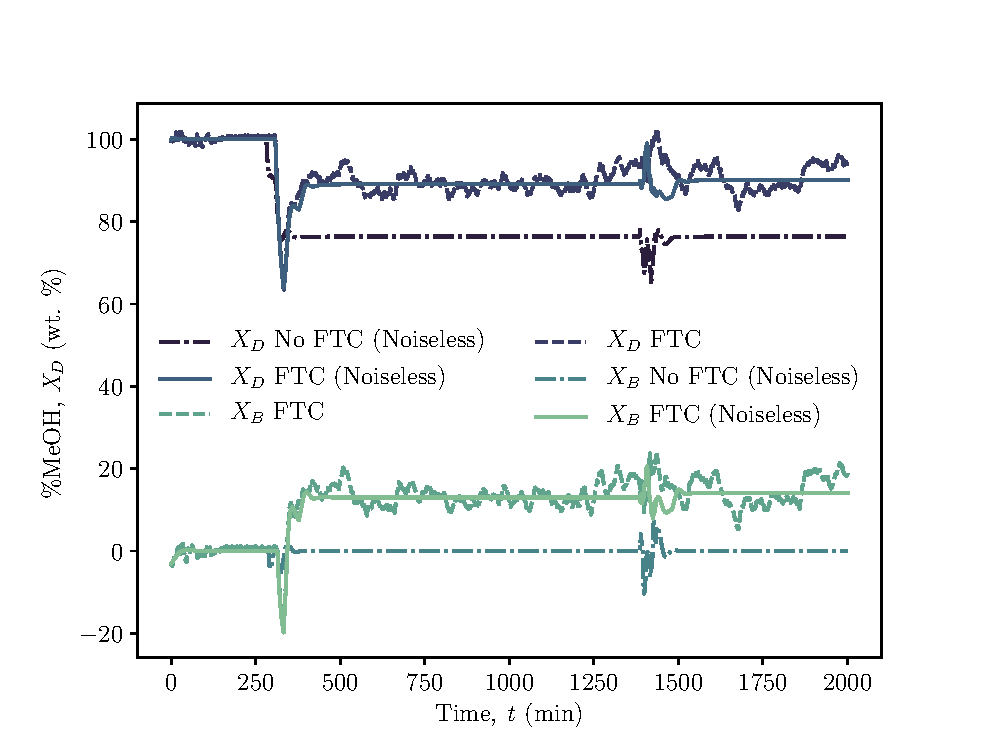
\includegraphics{images/ftc/Case3_Plot.eps}
        \caption{Trade-off between conflicting objectives (Case 3).}
        \label{fig:case_study3}
    \end{center}
\end{figure}

Case 4 was used to explore adaptability of the FTCS. A pre-trained control agent for regulating $X_D$ to 100 was re-tasked to regulate $X_B$ to 0.  In Fig. \ref{fig:case_study4}, a fault occurred at $t = 300$ in the reflux valve. Originally, the control agent was tasked with using the steam valve to regulate $X_D$ back to 100; however, the operating objective changed to regulating $X_B$ to 0. Here, the control agent was able to completely adapt to the new operating objective in 90,000 training steps by solely experiencing the new reward function. Adaptation speed can also be controlled by tuning learning rate $\alpha$.  

\begin{figure}[H]
    \begin{center}
        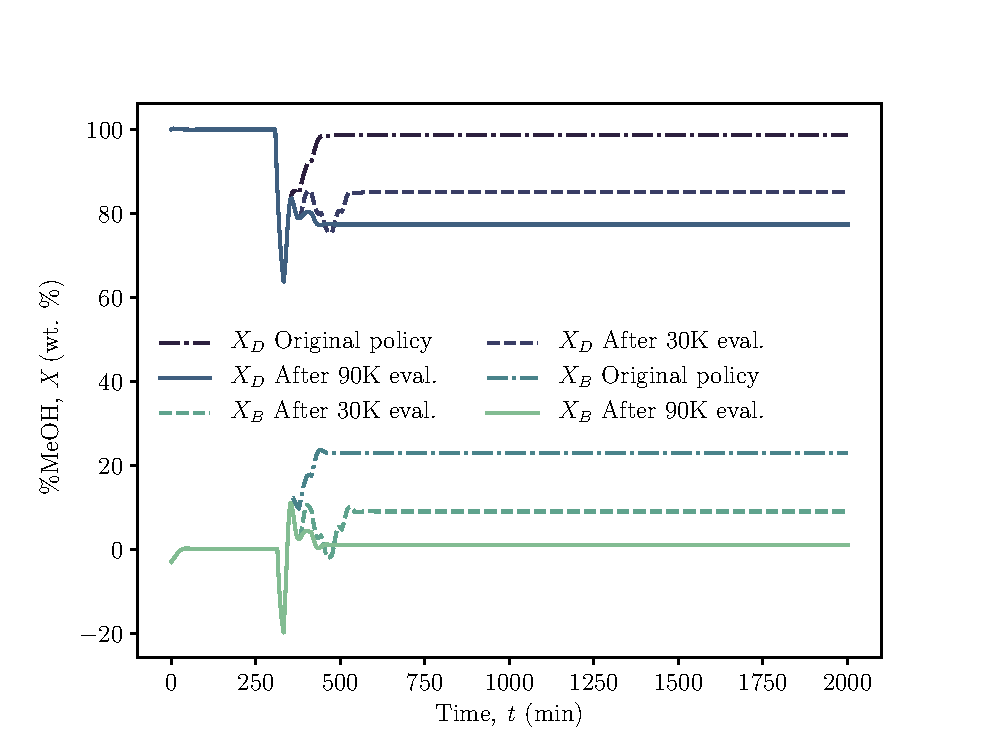
\includegraphics{images/ftc/Case4_Plot.eps}
        \caption{\label{fig:case_study4} Adaptation of the FTCS (Case 4).}
    \end{center}
\end{figure}

\subsection{Learning Speed and Fault Mediation Time}
Fig. \ref{fig:time_to_mediate} shows the time required to mediate faults of different magnitude. The fault mediation time was calculated as $t_{s} - t_{f}$, where $t_{s}$ is when the control agent made its first action and $t_f$ is when set points returned to 98\% of its original values.

From Fig. \ref{fig:time_to_mediate}, the time required to mediate a fault increased linearly with magnitude; however, this was caused by larger magnitude faults requiring additional actions from the control agent.  Moreover, the mediation time became constant after being normalizing by the minimum number of actions required to mediate the fault; the expected behaviour for linear systems. The control agent's actions can be increased to reduce mediation time during high magnitude faults.  Variance was higher at smaller magnitudes due to noise being more dominant.

Fig. \ref{fig:training_time} shows the control agent's performance for mediating a constant fault after different training steps. It can be seen that the mean performance does not greatly increase after 160,000 training steps; however, variance of results reduce significantly until 320,000  training steps.
\begin{figure}[H]
    \begin{center}
    \begin{subfigure}[b]{0.49\textwidth}
        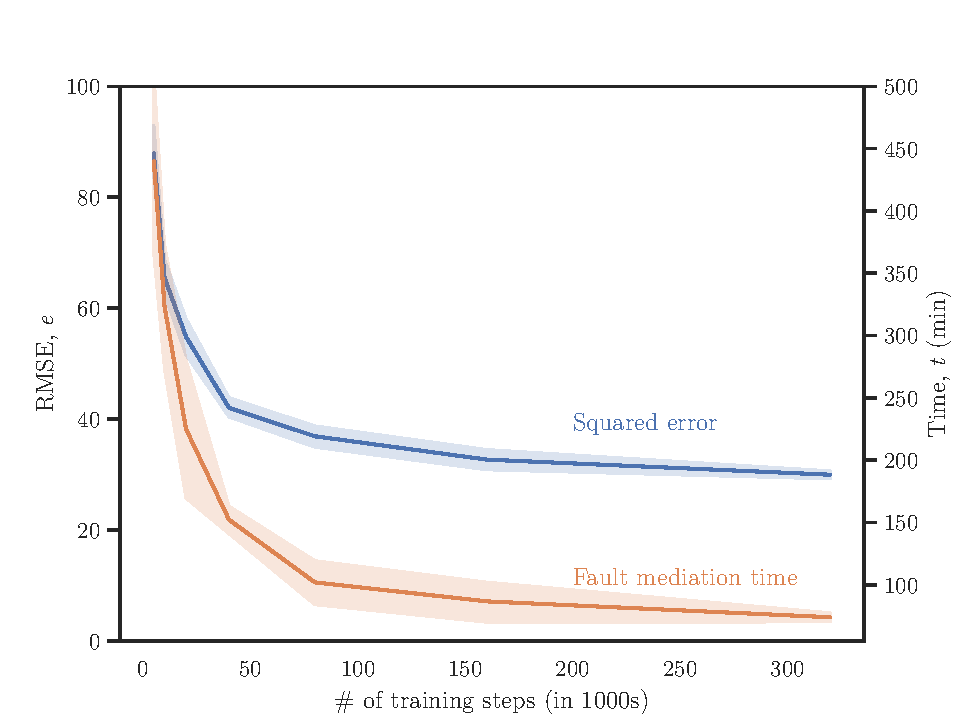
\includegraphics[width=\textwidth]{images/ftc/training_time.pdf}
        \caption{{\scriptsize Fault mediation time and error accumulation vs. \# of training steps averaged over 30 episodes. Shaded regions correspond to one standard deviation.}}
        \label{fig:training_time} 
    \end{subfigure}
    \begin{subfigure}[b]{0.46\textwidth}
        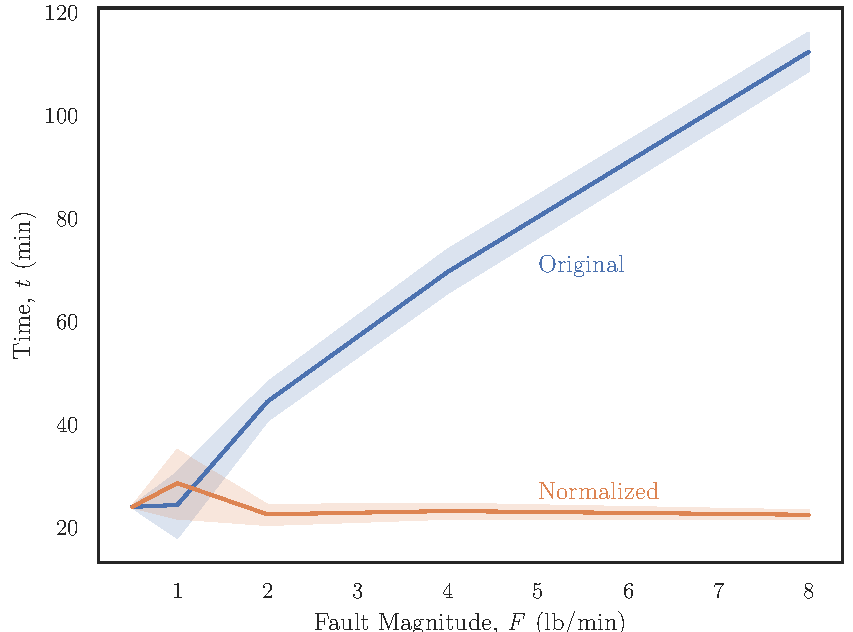
\includegraphics[width=\textwidth]{images/ftc/time_to_mediate.pdf}
        \caption{\label{fig:time_to_mediate} {\scriptsize Time required to mediate faults of different magnitudes averaged over 1000 simulations.  Shaded regions correspond to one standard deviation.}}
    \end{subfigure}
    \end{center}
\end{figure}

\subsection{A Comparison of Optimal Control}

In this section, the performance of the RL-FTCS was compared to MPC. A variety of factors relating to industrial implementation were explored for both MPC and RL under different situations. Factors include: performance, computational time, sensitivity to tuning, time required to implement, and robustness.

Figs. \ref{fig:ftcComparison} and \ref{fig:ftcRL_FTCS} show the $X_D$ trajectories under different control strategies during a fault. The strategies provided are:
\begin{enumerate}
    \item Classic MPC with no fault detection
    \item MPC equipped with the proposed FDS to detect faults
    \begin{enumerate}
        \item using a perfect model
        \item using a perfect model with un-tuned weighting matrices
        \item MPC using a model with 5\% mismatch 
    \end{enumerate}
    \item RL-FTCS
\end{enumerate}
For the MPC control strategies, the internal states of the system are all assumed to be measurable. The MPC cost function is given by:
\begin{equation}
        J = \sum\limits^{\infty}_{i=1} \gamma^i x_{i}^T Q x_{i} \\
\end{equation}
$$   x_{i} = x_i - x_i^{sp}$$
where $i$ denotes the stage number.  $\gamma = 0.9$ is the discount factor to decay future costs; a strategy RL uses to emphasize near-term performance. Here, it was added to the MPC's cost function to ensure the objective of both controllers are identical.  The control and prediction horizons for the MPCs are $\infty$; however, stage costs beyond $i = 50$ are decayed by 99.5\% due to $\gamma$. The MPC weighting matrix, $Q_{m \times m}$, is an identity matrix.  In the un-tuned MPC case, $Q_{m \times m}$ is a random diagonal matrix. Furthermore, the inputs of the MPC are bounded by $|u_i| \leq 10$, an identical condition imposed on the RL controller. Overall, the MPC's objective was designed to be an exact replica of the RL's reward function to ensure both controllers are solving identical problems.

\begin{figure}[H]
    \begin{center}
    \begin{subfigure}[b]{0.49\textwidth}
        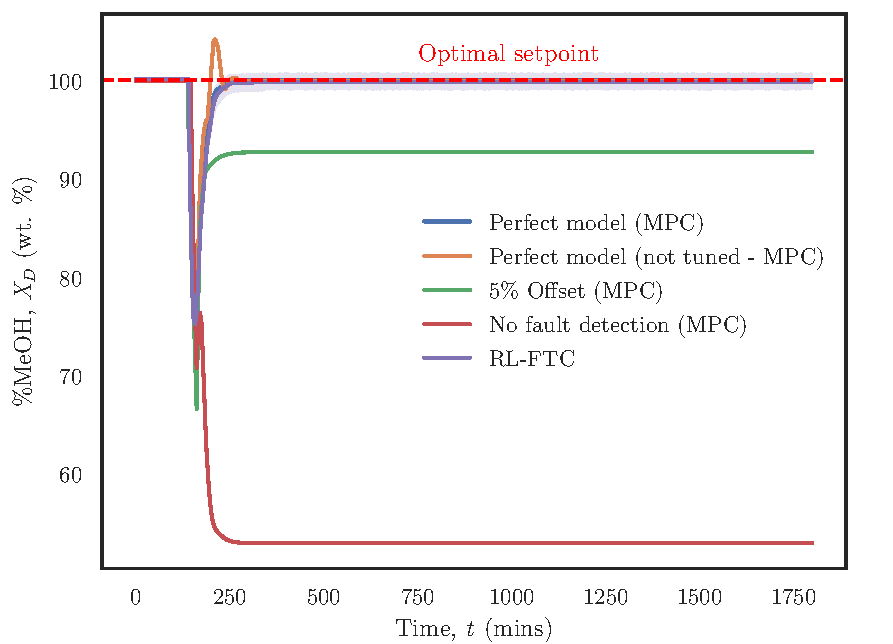
\includegraphics[width=\textwidth]{images/ftc/FTC_Comparison.pdf}
        \caption{{\scriptsize Trajectories of $X_D$ under different control strategies during a constant reflux valve fault. Shaded region correspond to one standard deviation.}}
        \label{fig:ftcComparison}
    \end{subfigure}
    \hfill
    \begin{subfigure}[b]{0.49\textwidth}
        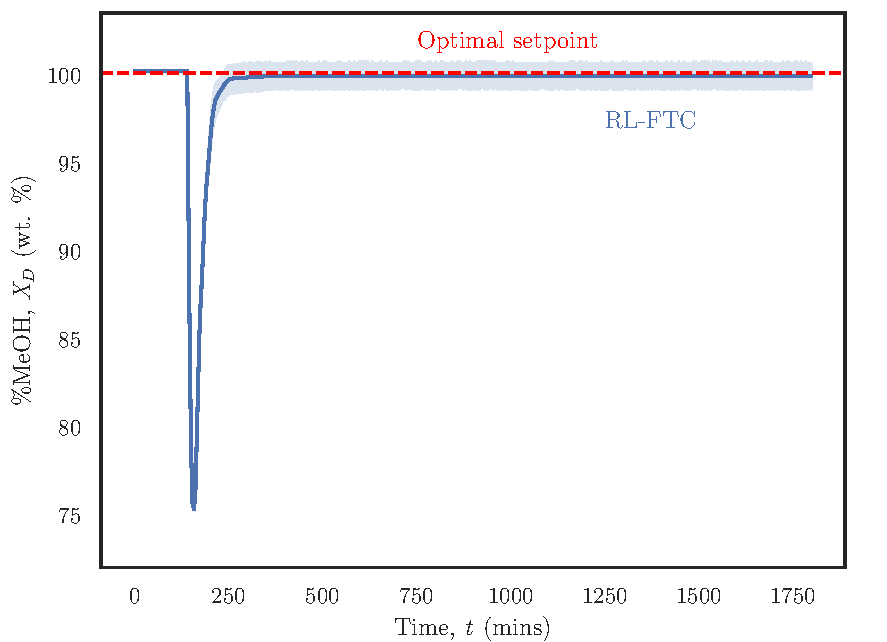
\includegraphics[width=\textwidth]{images/ftc/RL_FTC.pdf}
        \caption{{\scriptsize RL-FTC performance during a reflux valve fault averaged over 30 simulations.  RL-FTC was trained on a model with 5\% offset.}}
        \label{fig:ftcRL_FTCS}
    \end{subfigure}
    \end{center}
\end{figure}

In this simulation, a fault occurred in the reflux valve at $t = 350$, causing a major disturbance in $X_D$. For the MPC without fault detection, $X_D$ dropped drastically, and never recovered.  With the FDS equipped, the MPC with the \textbf{perfect} model was able to recover to pre-fault conditions very rapidly; however, the same MPC with a poorly tuned $Q$ matrix results in overshooting and sub-optimal performance.  Nevertheless, the fault was still rejected. However, for a MPC using a model with 5\% offset (all values in the A matrix are increased by 5\%), the MPC had a large offset and was never able to achieve pre-fault conditions due to the optimal trajectory calculated by the MPC being heavily reliant on the model itself.

Here, RL can overcome this problem through the velocity implementation style and its \textit{model-free} nature.  The RL in Fig. \ref{fig:ftcComparison} is trained on the 5\% offset model. But, RL uses the model only for an initial policy.  Afterwards, real-time feedback for RL is obtained in terms of an tracking error, $e_t$ from the plant, and does not rely on the initial model for any control purposes. Taking $e_t$, RL will perform control action $\Delta u$ with accordance to its current policy. Through this, RL was able to reject faults, even when trained on inaccurate models.  Additionally, RL will update its policy online to adapt to process drift, and continue to improve.

Table \ref{tab:08fault_performance} contains the performance metrics for the controllers shown in Fig. \ref{fig:ftcComparison}. MPC with a perfect model is still the superior choice, resulting in the lowest RMSE and fault mediation time.  On the contrary, if the weighting matrix is improperly tuned, the MPC's performance can suffer even using the perfect model.  RL (trained on the 5\% offset model) has higher RMSE and fault mediation time compared to MPC with a perfect model; however, RL performs better than all other MPC implementations, and will continue to improve when implemented online.
\begin{table}[H]
    \centering
    \def\arraystretch{1.1}
\begin{tabular}{ll|c|c}
                         &                          & RMSE & Mediation Time (mins) \\ \hline
\multicolumn{1}{c|}{}    & Perfect Model            & 21.6  & 46             \\
\multicolumn{1}{c|}{\rotatebox[origin=c]{90}{MPC}}  & Perfect Model (un-tuned) & 22.4  & 66             \\
\multicolumn{1}{c|}{} & 5\% Offset               & N/A  & $\infty$       \\
\multicolumn{1}{l|}{}    & No Fault Detection       & N/A  & $\infty$       \\ \hline
\multicolumn{1}{c|}{\rotatebox[origin=c]{90}{RL}}  & RL-FTC                   & 22.4  & 42            
\end{tabular}
    \caption{Performance metrics for fault mediation using different control strategies.}
    \label{tab:08fault_performance}
\end{table}

RL is also less prone to poor tuning as shown in Figs. \ref{fig:ftcAlpha} and \ref{fig:ftcBeta}, and only requires the output of the system for control.  For RL, the only hyper parameters that require tuning are $\alpha_{min}$ and $\beta$.  But from Figs. \ref{fig:ftcAlpha} and \ref{fig:ftcBeta}, it can be seen that RL is quite robust to poor hyper parameter tuning; a trait not exhibited by traditional optimal controllers. For $\alpha_{min}$, any values below 0.25 results in relatively the same performance.  Likewise for $\beta$, any values under 0.5 results in similar performance, with higher values only slightly depreciating performance.  Nevertheless, higher values result in significantly higher variance.

\begin{figure}[H]
    \begin{center}
    \begin{subfigure}[b]{0.49\textwidth}
        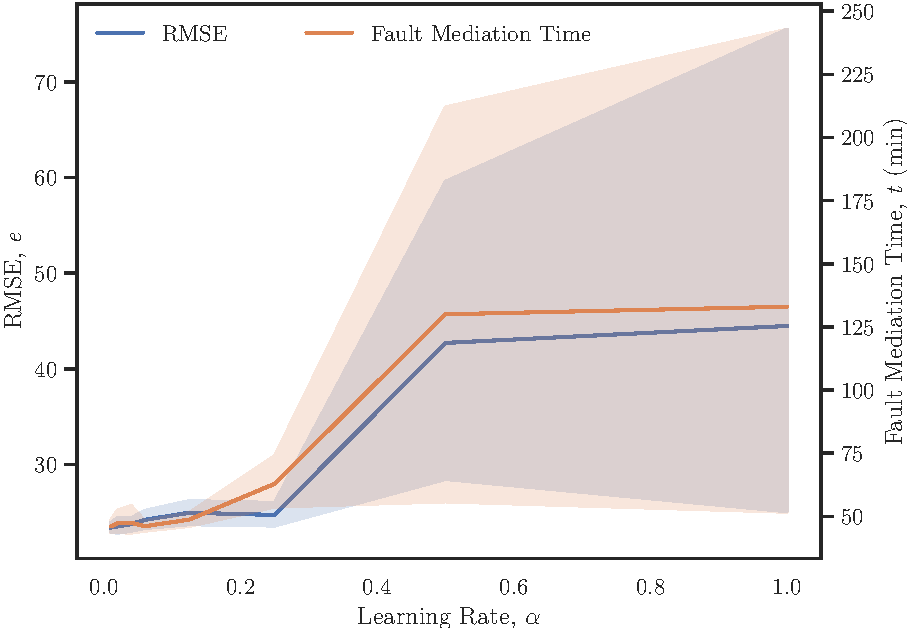
\includegraphics[width=\textwidth]{images/ftc/ftcAlpha.pdf}
        \caption{{\scriptsize RMSE and fault mediation time as a function of different fixed $\alpha$ during control agent training.}}
        \label{fig:ftcAlpha}
    \end{subfigure}
    \hfill
    \begin{subfigure}[b]{0.49\textwidth}
        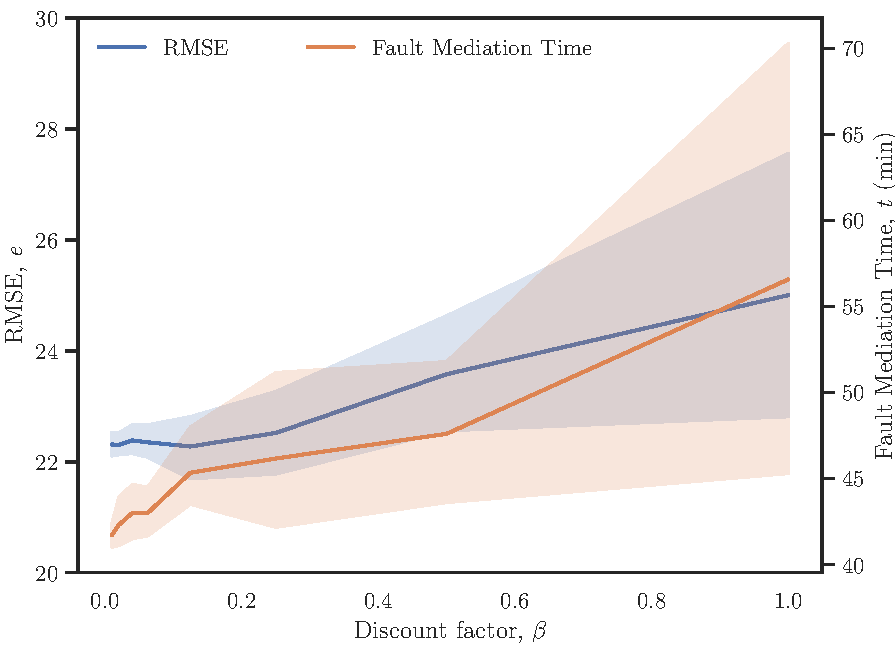
\includegraphics[width=\textwidth]{images/ftc/ftcBeta.pdf}
        \caption{{\scriptsize RMSE and fault mediation time as a function of different fixed $\beta$ during control agent training.}}
        \label{fig:ftcBeta}
    \end{subfigure}
    \end{center}
    \caption{Performance vs. $\alpha$ and $\beta$.  Solid line represent average performance of 10 different agents.  Shaded area represents one standard deviation.}
\end{figure}

The computational time of RL was also compared to MPC using IPOPT's linear program.  For a simulation lasting 2000 minutes, RL completed the simulation in 2.0 $\pm$ 0.2 \textbf{milliseconds} while MPC required 4.5 $\pm$ 0.1 seconds.  

Table \ref{tab:ftcAll} summarizes the performance of RL-FTC compared to traditional optimal controllers under actuator faults.

\begin{table}[H]
    \centering
    {\setstretch{1.1}
    \begin{tabular}{L|L|L}
                                 &   RL & MPC \\ \hline
$^1$RMSE                      & 22.4 & 21.6 \\
$^1$Mediation time (mins)     & 42 & 46 \\
$^2$Computational time (s)           & 0.002 $\pm$ 0.0002 & 4.5 $\pm$ 0.1 \\
Sensitivity to tuning            & No & Yes\\
Robustness                       & Yes & Bad models cause offset \\
Online calibration               & Exploratory moves & Exploratory moves \\
Requires offline training        & Yes & No \\ \hline
\multicolumn{3}{C{13.5cm}}{\scriptsize $^1$Lowest value achieved across all different simulations.  For RL, this value is the average of at least 10 simulations to ensure reproducability.} \\
\multicolumn{3}{C{13.5cm}}{\scriptsize $^2$Computational time required to run the Wood-berry distillation for 2000 minutes.}
    \end{tabular}}
    \caption{Summary of RL-FTC compared to MPC.}
    \label{tab:ftcAll}
\end{table}

\section{Concluding Remarks on the FTCS}
Eventually, all process equipment will reach the end of their operational lifetime and fail.  Such failures are difficult to predict and may cause catastrophic damage; therefore, it is advantageous to proactively manage risks using a fault-tolerant control system (FTCS).  This study proposed a general FTCS for continuous MIMO systems using reinforcement learning (RL). The FTCS was placed in the supervisory control layer and gave operating recommendations to process control systems. The FTCS was simulated distillation tower, showing its fault tolerant nature, robustness to uncertainties, and disturbance rejection capabilities all while being adaptive. The system was also evaluated from an industrial implementation perspective and compared to traditional optimal control methods similar to RL.  Unsurprisingly, MPC was found to be the superior method if a perfect model was provided and sufficient computational time was given. However, MPC falls short during scenarios with model plant mismatch, or if the controller is poorly tuned. RL's performance is only slightly worse than MPC, and is robust to model plant mismatch due to its \textit{model-free} nature and velocity implementation style. Ultimately, RL may be the preferred method in an industrial environment where hardware is lacking, engineers being under time pressure to create solutions, and/or fast computational time is necessary.

\section{Discussion: Cheaper, More Accurate, and Adaptive?}
\begin{itemize}
    \item \textbf{Cheaper: } training new operator - Training new operators - the first 6 months.
    \item \textbf{More Accurate: } aa
    \item \textbf{Adaptive: } aa
\end{itemize}
